\chapter{信号的表示与计算}
\label{chap:signal-analysis}

一段传感器记录既可以按时间逐项读取，也可以分解成不同频率的波动。
两种读法描述同一条信号，却适合回答不同问题：变化发生在何处，哪些振荡占主导，
一个局部滤波怎样作用，以及只保留部分样本后还能知道什么。这里需要分清三件事：
换一组完整坐标不一定丢失信息，滤波会改变信号，而采样会改变可用的观测。
计算某种表示很快，也不能代替对信息是否保留的判断。

本章沿用两个有限记录
\begin{equation}
  \bm x=(1,2,1),\qquad \bm h=(1,-1)
  \label{eq:signal-analysis-running-example}
\end{equation}
说明位置、边界、卷积与相关；需要非对称波形或连续时间时另行明确输入。
信号先作为带索引的函数出现，内积和范数给出共同的比较口径。
在此基础上，脉冲、复指数与多项式提供不同表示，输入输出映射说明如何改变信号，
采样条件则决定哪些区别仍能从观测中恢复。一般函数空间与线性坐标的背景可回查
第~\ref{chap:functional-analysis-and-approximation}章和第~\ref{chap:linear-algebra}章。
本章着重利用规则时间或位置索引；下一章再把位置之间的关系推广为一般图，
比较规则平移与图上传播的区别。至于怎样用内部状态产生输入输出响应，留给
第~\ref{chap:dynamical-systems-and-state-estimation}章。

\section{信号的对象与结构}
\label{sec:signal-objects-structure}

“三个数”还不是完整的信号说明。它们可能是三个时刻的温度，也可能是同一时刻
三个传感器的读数；数组首尾可能互不相连，也可能代表一个周期。
在比较大小或选择表示以前，需要先确定索引、取值和边界分别表示什么。

\subsection{信号的索引与取值}

\subsubsection{连续、离散与有限信号}

信号（signal）是定义在某个时间或位置索引集上的函数，函数值记录对应位置的量。
连续时间信号写成$x(t)$，离散时间信号写成$x[k]$；这里的“连续”描述索引，
不要求函数值随时间连续。例如发生突跳的开关读数仍是连续时间信号。

\begin{definition}[信号的索引类型]
  \label{def:signal-index-types}
  连续时间标量信号是$x:I\to\mathbb F$，其中$I\subseteq\mathbb R$为时间区间，
  $\mathbb F$取$\mathbb R$或$\mathbb C$。
  \term{离散时间信号}（discrete-time signal）是$x:\mathbb Z\to\mathbb F$，
  或定义在明确指定的整数子集上。长度$N$的有限信号是
  $x:\{0,\ldots,N-1\}\to\mathbb F$，可按位置写成$\bm x\in\mathbb F^N$。
\end{definition}

数组下标只是位置编号。若第$k$项来自时刻$t_0+kT_s$，还要给出起点$t_0$及间隔
$T_s$，才能把“每两项一次振荡”换算成物理频率。不等间隔观测则需要显式保存每个
时间戳，不能直接套用均匀采样公式。二维图像以两个整数坐标标位置，规则网格上的
运算可以相应推广到$\mathbb Z^d$，但一般图节点的编号不自带这种平移结构。

有序信号与无序样本集合也不同。$(1,2,1)$和$(1,1,2)$有同样的取值及重数，
相邻变化却不同，因此局部差分或模板比较可以区分它们。
随机信号则是在概率空间上给每个索引配一个随机变量；固定一次随机结果$\omega_0$
后，$k\mapsto X_k(\omega_0)$成为一条确定路径。对这条路径求频谱与对随机信号求
期望是不同操作，一次观察不自动给出总体规律。本章先研究给定的确定信号，
随机变量、过程及期望在第~\ref{chap:random-variables}章建立后再用于随机信号。

复数值常用来同时记录两个实分量或表示振荡的幅度与相位。
记$\mathrm i^2=-1$，对$z=a+\mathrm ib$有
$\overline z=a-\mathrm ib$、$|z|^2=z\overline z=a^2+b^2$。
这里的\term{复共轭}（complex conjugate）只改变虚部符号，不是时间反转；
后文内积中的共轭正是为了使自内积得到非负的大小。

\subsubsection{单通道与多通道信号}

立体声在同一时刻有左右两路读数。将两路首尾接起来会把通道差别误当成时间先后，
因此需要分别记录这两种索引。
\begin{definition}[标量信号与向量值信号]
  \label{def:signal-multichannel}
  单通道信号在每个位置取一个标量值。$d$通道信号在每个位置取向量值
  $\bm x[k]=(x_1[k],\ldots,x_d[k])^\top\in\mathbb F^d$；
  连续时间时相应写作$\bm x(t)$。
  $N$个位置的记录可写为$\bm X\in\mathbb F^{N\times d}$，
  约定$\bm X_{k+1,c}=x_c[k]$，其中$k=0,\ldots,N-1$、$c=1,\ldots,d$。
\end{definition}

时间轴长度为$N$，通道数为$d$，两者不互换。比如
\begin{equation}
  \bm X=
  \begin{bmatrix}1&0\\2&1\\1&2\end{bmatrix}
  \label{eq:signal-multichannel-record}
\end{equation}
有三个时刻、两个通道；第二行$(2,1)$是同一时刻的联合读数。
把两个传感器放在同一个向量里，隐含它们已经按同一时间基准对齐；若第二通道延迟
一个采样间隔，应先保留这一偏移，不能把不同时刻的值当作同时观测。
多通道既不意味着通道独立，也不意味着必须逐通道处理：
可以对每一列分别滤波，也可以在每个时刻以矩阵混合多个通道。
后者的输入输出维度及时间作用将在第~\ref{sec:signal-input-output-maps}节明确区分。

\subsection{信号的周期与边界}

\subsubsection{周期信号与非周期信号}

重复观察到相似波形不等于已经证明周期性。周期要求整个定义域上的精确重复，
还要求每次平移都留在允许的索引内。
\begin{definition}[周期及基本周期]
  \label{def:signal-period}
  定义在$\mathbb R$上的信号$x$若存在$T>0$使$x(t+T)=x(t)$对所有$t$成立，
  则称其为周期信号，$T$为一个周期。
  定义在$\mathbb Z$上的信号若存在正整数$N$使$x[k+N]=x[k]$对所有整数$k$成立，
  则称其为周期序列。若正周期中存在最小者，才称其为基本周期。
  没有正周期的信号称为非周期信号。
\end{definition}

在按几乎处处相等识别函数的空间中，周期等式也按几乎处处理解。
常数连续信号的每个正实数都是周期，却没有最小正周期；
离散周期的候选是正整数，非空时一定有最小者。
连续复指数$e^{\mathrm i\Omega t}$在$\Omega\neq0$时有基本周期
$2\pi/|\Omega|$；离散复指数$e^{\mathrm i\omega k}$则要求
$e^{\mathrm i\omega N}=1$，即$\omega/(2\pi)$为有理数，才有整数周期。
所以连续振荡取样后是否周期还取决于取样间隔与振荡周期的比例。

多通道周期要求所有通道具有一个共同周期。例如
\[
  \bm x(t)=\begin{pmatrix}\cos t\\\cos(\sqrt2\,t)\end{pmatrix}
\]
的每一分量都周期，
但共同周期必须同时满足$T=2\pi m$和$\sqrt2 T=2\pi n$，
其中$m,n$为整数；无理数$\sqrt2$使正$T$不可能存在。
离散的有限多个周期通道则可取各整数周期的最小公倍数作为共同周期。

还应区分三个对象：物理信号本来周期，有限数组被人为周期延拓，
以及变换所得频谱以某个频率间隔重复。DFT可以给任意有限数组配置循环索引，
不要求记录前后的真实过程恰好重复；DTFT的频率周期来自整数时间索引，
也不要求原序列周期。这些区别会决定后文“回绕”发生在时间轴还是频率轴。

\subsubsection{有限支撑与边界延拓}

有限记录只说明观测范围。为了计算跨过首尾的运算，还必须说明区间外采用什么值。
离散信号的支撑是$\{k:x[k]\neq0\}$；只有有限个非零位置时称为有限支撑。
连续信号通常以非零集合的闭包定义支撑，$L^p$类中使用忽略零测差别的本质支撑。
连续时间的有限支撑在此指支撑包含于某个有界区间，不是只有有限个非零点。

对$x[0],\ldots,x[N-1]$，零延拓令区间外的值为零；
周期延拓令$x[k]=x[k\bmod N]$；反射延拓则把边界附近的值镜像放到区间外。
反射有不同端点约定。例如不重复端点且$N\geq2$时，
$x[-1]=x[1]$、$x[N]=x[N-2]$，再以$2(N-1)$为周期延续；
若重复端点，就有$x[-1]=x[0]$、$x[N]=x[N-1]$，得到另一个延拓。
两种方式都可能合理，但不是同一个输入。

贯穿例$(1,2,1)$零延拓后，左边相邻值为$0$；周期延拓时为$1$；
不重复端点的反射延拓时为$2$。在位置$0$计算当前值减前值，三者分别得到
$1,0,-1$。这个差别出现在运算之前，不能由之后采用哪种快速算法来决定。

输出裁剪又是另一项选择：先按给定延拓计算输出，再只保留指定位置。
裁去首尾不等于改变输入延拓，保持输出长度也不能唯一决定左右怎样补值。
周期索引上的运算只在一个周期内计数；若把两条周期延拓序列直接在整轴上无穷求和，
同一个贡献会重复无穷次。这一边界将在循环卷积的定义中保留。

\subsection{信号的比较与大小}

\subsubsection{基于内积的信号比较}

判断两个记录是否接近，需要决定哪些位置和通道参与比较。
第~\ref{chap:functional-analysis-and-approximation}章使用实内积；
本章扩展到复信号时采用第一变量线性、第二变量取共轭的约定。
它与第~\ref{sec:linear-algebra-length-angle-distance}节的复坐标约定互为共轭，
实信号时两者相同；范数与正交性不变，读取展开系数时却要相应调整内积的顺序。
对有限记录、平方可和序列与平方可积函数，分别有
\begin{equation}
  \begin{aligned}
    \langle x,z\rangle_N&=\sum_{k=0}^{N-1}x[k]\overline{z[k]},\\
    \langle x,z\rangle_{\ell_2}&=\sum_{k\in\mathbb Z}x[k]\overline{z[k]},\\
    \langle x,z\rangle_{L^2}&=\int_{\mathbb R}x(t)\overline{z(t)}\,\mathrm dt.
  \end{aligned}
  \label{eq:signal-inner-products}
\end{equation}
后两式的乘积由Cauchy--Schwarz不等式保证绝对可和或绝对可积。
内积为零表示在当前比较口径下正交，诱导距离为$\|x-z\|_2$。
非零信号的归一化比较量
$\rho(x,z)=\langle x,z\rangle/(\|x\|_2\|z\|_2)$满足$|\rho|\leq1$；
实信号时这是夹角余弦，复信号时它一般是复数，包含相对相位。
零信号没有这种归一化相似性，不能直接除以零。

例如$x=(1,2,1)$、$z=(1,0,-1)$满足$\langle x,z\rangle=0$，
但两者在位置$0$都有非零值。正交描述汇总贡献抵消，不要求支撑互不相交。
若把$x$变成$2x$，归一化相似性仍为$1$，距离却为$\|x\|_2$；
这说明方向相同与数值接近是两个判断。

多通道内积同时汇总位置与通道：
\[
  \langle\bm x,\bm z\rangle
  =\sum_k\sum_{c=1}^d x_c[k]\overline{z_c[k]}.
\]
如果不同传感器的单位或重要性不同，可明确选正权重$w_c$，
把每项乘以$w_c$。更一般地，Hermitian正定矩阵$\bm W$给出
$\sum_k\bm z[k]^*\bm W\bm x[k]$，其中$*$表示共轭转置。
正定性使非零信号的自内积为正；仅半正定时某些非零通道组合可能被忽略。
改变权重可能改变正交关系及相似性排序，不能把它当作不影响结论的单位装饰。

\subsubsection{基于范数的信号大小}

峰值关心某一时刻是否过大，绝对累计关心全部幅值的总量，平方累计更强调大幅值。
对离散标量信号，相应范数是
\[
  \|x\|_\infty=\sup_k|x[k]|,\qquad
  \|x\|_1=\sum_k|x[k]|,\qquad
  \|x\|_2=\left(\sum_k|x[k]|^2\right)^{1/2}.
\]
在有限记录上求和只取记录范围；整轴上则要求相应总和有限。
记$\ell_1(\mathbb Z)$为绝对可和序列空间，$\ell_2(\mathbb Z)$为平方可和序列空间。
例如$x[k]=(k+1)^{-1}$在$k\geq0$时取此值、在$k<0$时取零，
属于$\ell_2$却不属于$\ell_1$。所以可以定义能量的信号未必能直接使用
绝对收敛的变换或卷积论证。

连续情形将和换成积分，得到$L^1$与$L^2$范数；$L^\infty$采用
$\operatorname*{ess\,sup}_t|x(t)|$，即忽略零测异常点后的最小本质上界。
这不同于最大值：函数可能只趋近其上界而未取到，也可能在单个点被赋任意大值，
但代表同一个$L^\infty$元素。真实采样要读取点值，届时必须另行确定代表元。

对贯穿有限记录，$\|x\|_\infty=2$、$\|x\|_1=4$、$\|x\|_2=\sqrt6$。
重排位置不改变这三个数，却可以改变局部波形；范数不是完整的形状描述。
多通道的二范数可按
$\|\bm x\|_2^2=\sum_k\|\bm x[k]\|_2^2$定义，
若使用前述$\bm W$，则改为$\sum_k\bm x[k]^*\bm W\bm x[k]$。
比较前须固定通道度量，不能把不同单位的读数无说明地相加。

\subsubsection{有限能量与平均功率}

持续振荡的幅值可以有界，但持续时间无限，平方累计仍会发散。
这时需要区分累计了多少与每单位时间平均有多少。
\begin{definition}[信号能量与平均功率]
  \label{def:signal-energy-power}
  离散及连续信号的能量分别为
  \[
    E_x=\sum_{k\in\mathbb Z}|x[k]|^2,\qquad
    E_x=\int_{\mathbb R}|x(t)|^2\,\mathrm dt.
  \]
  能量有限等价于属于相应的$\ell_2$或$L^2$空间，且$E_x=\|x\|_2^2$。
  长期平均功率在相应极限存在时定义为
  \begin{align*}
    P_x&=\lim_{K\to\infty}\frac1{2K+1}\sum_{k=-K}^K|x[k]|^2,\\
    P_x&=\lim_{R\to\infty}\frac1{2R}\int_{-R}^R|x(t)|^2\,\mathrm dt.
  \end{align*}
\end{definition}

这里是以幅值平方定义的信号指标；若要解释为物理能量或功率，还需相应单位与系统系数。
窗口能量则只在声明的记录窗口求和或积分。
贯穿例零延拓后的能量为$6$；若将它按周期$3$延拓，单周期能量仍为$6$，
平均功率却为$6/3=2$，整轴能量发散。
一般周期序列满足$P_x=N^{-1}\sum_{k=0}^{N-1}|x[k]|^2$，
局部平方可积的$T$周期函数满足$P_x=T^{-1}\int_0^T|x(t)|^2\,\mathrm dt$。
两式可由长窗口分成完整周期与长度有界的剩余段得到。

非零正弦$x(t)=A\cos(\Omega t+\varphi)$在$\Omega\neq0$时，
利用$\cos^2 u=(1+\cos2u)/2$得到一个周期的平方积分为$A^2T/2$，
故$P_x=A^2/2$，而无限多个周期的累计能量为无穷。
相反，有限能量信号的长期平均功率为零，因为平均的分子不超过总能量，
分母却趋于无穷。非周期有界信号未必有平均功率极限，例如让取值$0$和$1$的
交替时间块各自长到压过此前全部时间，窗口平均就可能持续在不同水平间变化。

后文Parseval关系只是在另一组坐标下计算这里已经定义的能量或周期平均功率。
其中出现$N$、$T$或$2\pi$的尺度因子来自变换与内积的归一化，
不是同一条信号在换坐标后获得了更多能量。

\section{信号的表示与分解}
\label{sec:signal-analysis-frequency-representation}

直接记录每个位置的值，最容易回答“变化发生在哪里”；要判断一条记录由哪些振荡组成，
则需要另一组坐标。表示的任务是描述同一对象，而不是先改变它。
下面先用脉冲分离位置贡献，再用复指数分离振荡模式，最后把有限序列改写为多项式。
每次转换都要说明哪些坐标足以恢复原信号，以及无穷展开按何种意义收敛。

\subsection{时域表示与脉冲分解}
\label{sec:signal-time-impulses}

把一个读数放回它原来的位置，可以用“仅在该位置为一”的信号来完成。
对整数$r$，约定平移算子为
\[
  (T_rx)[k]=x[k-r].
\]
$r>0$时，原来位于$k$的值移动到$k+r$，因而表示延迟。
单位脉冲定义为
\[
  \delta[k]=
  \begin{cases}
    1,&k=0,\\
    0,&k\neq0.
  \end{cases}
\]
于是$T_r\delta[k]=\delta[k-r]$只在位置$r$非零。任意有限支撑信号都有展开
\begin{equation}
  x[k]=\sum_{r\in\mathbb Z}x[r]\delta[k-r].
  \label{eq:signal-analysis-impulse-expansion}
\end{equation}
例如贯穿输入就是$\delta[k]+2\delta[k-1]+\delta[k-2]$。
对每个固定$k$，只有$r=k$的一项留下；对有限支撑输入，整个表达还是有限和。
后文系统若允许叠加，就可分别计算这些脉冲的输出再相加。

有限记录上的各位置脉冲是标准正交基，系数恰好是原读数，完整展开不会丢失信息。
若只保留位置集合$S$，得到$x_S[k]=x[k]\mathbb I_S(k)$，则
\[
  \|x-x_S\|_2^2=\sum_{k\notin S}|x[k]|^2.
\]
这才是投影近似：未保留的位置进入误差。对$x=(1,2,1)$只保留中间位置，
近似为$(0,2,0)$，平方误差为$2$。保留一个时域系数与保留一个频域系数，
舍弃的是不同方向，不能仅按系数个数比较误差。
对$x\in\ell_2$，对称截断$\sum_{|r|\leq K}x[r]T_r\delta$在$\ell_2$中趋于$x$；
这是尾部平方和趋零的结果，不是对任意信号都成立的无条件范数收敛。

\subsection{频域表示与傅里叶分解}

脉冲在平移后换了位置，复指数却保持形状。对
$\phi_\omega[k]=e^{\mathrm i\omega k}$有
\[
  (T_r\phi_\omega)[k]
  =e^{\mathrm i\omega(k-r)}
  =e^{-\mathrm i\omega r}\phi_\omega[k].
\]
平移只乘上模长为一的系数，因此这些振荡是平移算子的特征模式。
频率$\omega$区分振荡快慢，系数的相角记录时间原点变化。
这给出选择频率坐标的动机；具体用有限和、无穷级数还是积分，
仍由时间索引及周期条件决定。以下离散公式以$n$记时间位置、$k$记频率格。

\subsubsection{有限离散信号的傅里叶表示}

长度$N$的有限记录若采用循环索引，允许的复指数必须在移动$N$格后回到原值。
因此频率取$2\pi k/N$。令$\omega_N=e^{-2\pi\mathrm i/N}$。
\begin{definition}[离散傅里叶变换]
  \label{def:signal-analysis-dft}
  对$N\geq1$及$x\in\mathbb C^N$，\term{离散傅里叶变换}
  （discrete Fourier transform, DFT）及逆变换为
  \begin{align}
    \widehat x[k]&=\sum_{n=0}^{N-1}x[n]\omega_N^{kn},
    &&k=0,\ldots,N-1,
    \label{eq:signal-analysis-dft}\\
    x[n]&=\frac1N\sum_{k=0}^{N-1}\widehat x[k]\omega_N^{-kn},
    &&n=0,\ldots,N-1.
    \label{eq:signal-analysis-idft}
  \end{align}
\end{definition}
循环索引是这组基的边界条件，不是对真实观测过程永久重复的断言。
逆公式的依据是单位根正交关系：对整数$n,s$，
\begin{equation}
  \sum_{k=0}^{N-1}\omega_N^{k(n-s)}
  =
  \begin{cases}
    N,&n\equiv s\pmod N,\\
    0,&n\not\equiv s\pmod N.
  \end{cases}
  \label{eq:signal-analysis-root-orthogonality}
\end{equation}
第一种情形每项都是$1$。第二种情形令$q=\omega_N^{n-s}\neq1$，则$q^N=1$，
几何级数给出$(1-q^N)/(1-q)=0$。将正变换代入逆变换，直接得到
\[
  \frac1N\sum_{k=0}^{N-1}\sum_{s=0}^{N-1}x[s]\omega_N^{k(s-n)}
  =\sum_{s=0}^{N-1}x[s]\mathbb I_{\{s=n\}}=x[n].
\]
两次求和都是有限和，没有交换极限的问题；这证明全部$N$个系数能精确恢复记录。
只保留其中一部分则是另一项截断操作。

记DFT矩阵为$\bm F$，$F_{k+1,n+1}=\omega_N^{kn}$。
矩阵的\term{共轭转置}（conjugate transpose）为
$\bm F^*=\overline{\bm F}^{\top}$，正交关系给出$\bm F^*\bm F=N\bm I$，
所以$\bm F/\sqrt N$才是酉矩阵。由此
\[
  \|\widehat{\bm x}\|_2^2
  =\bm x^*\bm F^*\bm F\bm x=N\|\bm x\|_2^2,
\]
得到本章归一化下的\term{Parseval关系}
\begin{equation}
  \sum_{n=0}^{N-1}|x[n]|^2
  =\frac1N\sum_{k=0}^{N-1}|\widehat x[k]|^2.
  \label{eq:signal-analysis-parseval}
\end{equation}
正逆变换若各用$1/\sqrt N$，等式便没有额外因子。多通道DFT逐通道变换时，
对各通道的等式求和就得到总能量关系，不把通道数误当作变换长度。

每个非零系数可写成$\widehat x[k]=|\widehat x[k]|e^{\mathrm i\arg\widehat x[k]}$。
模长是该频率坐标的大小，相角是相对于时间原点的相位；它不是直接等于实余弦的峰值，
还要考虑正负频率配对和$1/N$归一化。循环平移$r$格后，换元得到
\[
  \widehat{T_rx}[k]=\omega_N^{kr}\widehat x[k].
\]
因此幅度不变，相位随$k$线性改变。若只保存幅度，便不能区分这些位置不同的信号。
零系数没有确定的相角，软件为它返回的角度不携带波形信息。

实信号还具有\term{共轭对称}（conjugate symmetry），因为
\[
  \overline{\widehat x[k]}
  =\sum_{n=0}^{N-1}x[n]\omega_N^{-kn}
  =\widehat x[(N-k)\bmod N].
\]
$k=0$的系数总是实数；$N$为偶数时，$k=N/2$对应交替变号模式$(-1)^n$，
其离散角频率$\pi$称为Nyquist频率，该处系数也为实数。
其余频率成对出现，使用单边频谱时必须说明这两个端点是否加倍。

例如$x[n]=\cos(2\pi n/8)$只在$k=1,7$有非零DFT系数，二者都为$4$；
延迟两格的$z[n]=x[(n-2)\bmod8]$在这两处变为$-4\mathrm i$与$4\mathrm i$。
两条信号的能量都为$4$，也等于$(4^2+4^2)/8$。
图~\ref{fig:signal-amplitude-phase}在同一频率顺序下比较幅度和相位，帮助分清
“含有相同频率强度”与“具有相同波形”。
\begin{figure*}[htbp]
  \centering
  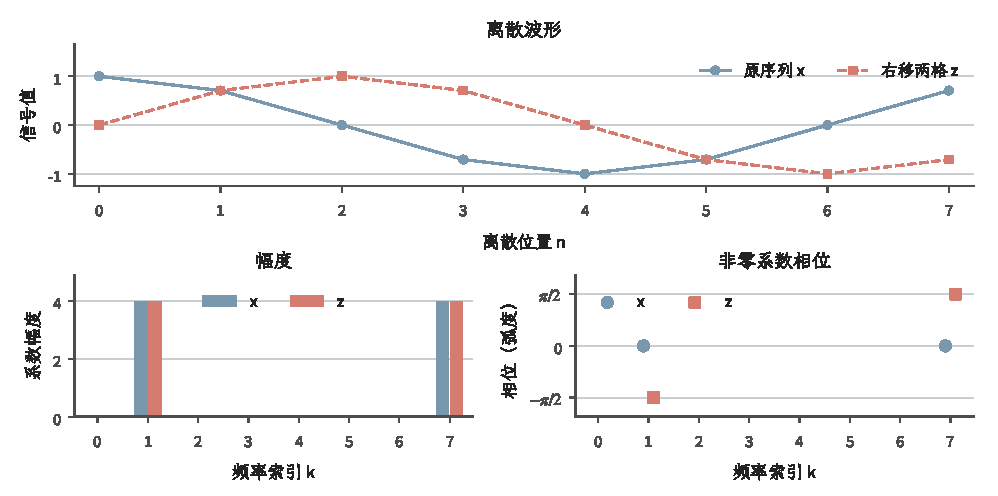
\includegraphics[width=\linewidth]{figures/01-mathematical-preliminaries/03-graphs-and-signals/matplotlib/concepts-dynamics/amplitude-phase.pdf}
  \caption{长度$8$的教学信号$x[n]=\cos(2\pi n/8)$及其循环延迟两格的结果。
  上方波形的峰值位置不同，下方在$k=1,7$的幅度均为$4$，相位却改变。
  相位图只画非零系数；波形连线只帮助观察顺序，不表示已选择连续时间插值。}
  \label{fig:signal-amplitude-phase}
\end{figure*}

这里的复指数坐标来自规则循环平移：每次移动都有统一的方向和步长，DFT同时分解
这些平移。如果位置只通过不规则的连接关联，就不能再根据编号判断谁是“下一格”。
第~\ref{sec:signal-analysis-graph-state-kernels}节将用图上的连接定义变化，
并通过环图说明本节的复指数怎样成为图谱的一个特例。

\subsubsection{周期连续信号的傅里叶表示}

连续时间的一个周期含无穷多个位置，有限个坐标一般不足以完整描述。
周期条件仍把频率限制在整数谐波上，但展开变为无穷级数。
\begin{definition}[周期信号的傅里叶系数与级数]
  \label{def:signal-analysis-fourier-series}
  设$T>0$，$f\in L^2[0,T]$并按周期$T$延拓。在内积
  \[
    \langle f,g\rangle_T=\frac1T\int_0^T f(t)\overline{g(t)}\,\mathrm dt
  \]
  下，复指数$e^{\mathrm i2\pi kt/T}$组成正交归一基。
  \term{傅里叶系数}（Fourier coefficient）为
  \[
    c_k=\frac1T\int_0^T f(t)e^{-\mathrm i2\pi kt/T}\,\mathrm dt,
    \qquad k\in\mathbb Z,
  \]
  相应傅里叶级数写作
  \begin{equation}
    f(t)\sim\sum_{k\in\mathbb Z}c_ke^{\mathrm i2\pi kt/T}.
    \label{eq:signal-analysis-fourier-series}
  \end{equation}
\end{definition}
正交性由对$e^{\mathrm i2\pi(k-j)t/T}$积分得到：$k=j$时归一化积分为$1$，
否则两个端点的指数相同，积分为$0$。完备性给出对称部分和
$S_Kf=\sum_{|k|\leq K}c_ke^{\mathrm i2\pi kt/T}$的$L^2$收敛，
即$T^{-1}\int_0^T|S_Kf-f|^2\to0$。它描述一个周期的平均平方误差，
不能单凭这一结论就在每个$t$写逐点等号。

由正交展开及其极限得到
\begin{equation}
  \frac1T\int_0^T|f(t)|^2\,\mathrm dt
  =\sum_{k\in\mathbb Z}|c_k|^2.
  \label{eq:signal-analysis-continuous-parseval}
\end{equation}
左侧是周期平均功率；单周期能量还要乘以$T$，整轴能量通常无穷。
相应截断误差为$\sum_{|k|>K}|c_k|^2$。
实信号满足$c_{-k}=\overline{c_k}$，延迟$\tau$则把$c_k$变为
$e^{-\mathrm i2\pi k\tau/T}c_k$，幅相的作用与有限情形相同。

逐点重构需增加规则性。例如在一个周期内分段$C^1$、只有有限个跳跃点且单侧极限
存在时，傅里叶级数在连续点趋于$f(t)$，在跳跃点趋于左右极限平均。
这是带条件的结论；不能把均方收敛与逐点或一致收敛互换，
相关性质保持条件可回查第~\ref{chap:mathematical-analysis}章。

取周期$2\pi$的方波：$0<t<\pi$时为$1$，$-\pi<t<0$时为$-1$。
平均值$c_0=0$；对$k\neq0$直接积分，
\[
  c_k=\frac1{2\pi}\left(
    \int_0^\pi e^{-\mathrm ikt}\,\mathrm dt
    -\int_{-\pi}^0 e^{-\mathrm ikt}\,\mathrm dt\right)
  =\frac{1-(-1)^k}{\pi\mathrm ik}.
\]
因此偶数$k$的系数为零，奇数$k$的系数为$2/(\pi\mathrm ik)$，也可配对写成
\[
  \frac4\pi\left(\sin t+\frac{\sin3t}{3}+\frac{\sin5t}{5}+\cdots\right).
\]
连续点处恢复$\pm1$，跳跃点处趋于$0$，无论给原函数的跳跃点赋什么值，
其$L^2$元素和傅里叶系数都不变。Parseval仍给出
$1=(8/\pi^2)\sum_{j=0}^{\infty}(2j+1)^{-2}$。
平均平方误差趋零并不排除跳跃附近的局部振荡；这也是有限谐波近似尖锐边沿时
需要单独观察局部误差的原因。

\subsubsection{整轴离散信号的傅里叶表示}

一条整轴序列不必周期，频率也不再局限于$N$个格点。
但整数$n$使$e^{-\mathrm i(\omega+2\pi)n}=e^{-\mathrm i\omega n}$，
因此频率变量虽然连续，频率表示仍以$2\pi$为周期。
\begin{definition}[离散时间傅里叶变换]
  \label{def:signal-analysis-dtft}
  对$x\in\ell_1(\mathbb Z)$，\term{离散时间傅里叶变换}
  （discrete-time Fourier transform, DTFT）定义为
  \begin{equation}
    X(e^{\mathrm i\omega})=\sum_{n\in\mathbb Z}x[n]e^{-\mathrm i\omega n},
    \qquad \omega\in\mathbb R.
    \label{eq:signal-analysis-dtft}
  \end{equation}
  绝对可和使级数绝对且一致收敛，因而定义连续的$2\pi$周期函数。
\end{definition}
记号$X(e^{\mathrm i\omega})$强调只沿单位圆取值，不在这里假设存在一般复变量的
解析延拓。对$x\in\ell_2$，相同级数改按$L^2([-\pi,\pi])$收敛解释，
所得对象是等价类，不要求每个$\omega$都能按普通级数求值。
两种情形均有系数恢复与能量关系
\begin{align*}
  x[n]&=\frac1{2\pi}\int_{-\pi}^{\pi}
  X(e^{\mathrm i\omega})e^{\mathrm i\omega n}\,\mathrm d\omega,\\
  \sum_n|x[n]|^2&=\frac1{2\pi}\int_{-\pi}^{\pi}|X(e^{\mathrm i\omega})|^2\,\mathrm d\omega.
\end{align*}
在$\ell_1$情形可把绝对收敛级数移入积分，单位复指数的正交性留下第$n$项；
$\ell_2$情形则来自周期$L^2$空间的正交基与Parseval关系。

贯穿例零延拓后的DTFT为
$X(e^{\mathrm i\omega})=1+2e^{-\mathrm i\omega}+e^{-2\mathrm i\omega}$，
它是连续频率曲线。对$N\geq3$，将记录补零到$N$项后计算DFT，
只是读取这条曲线在$\omega=2\pi k/N$上的值。补更多零增加了频率格密度，
没有增加原记录的信息或延长真实观测。
相反，若原序列无穷长，先截取$N$项再作DFT，频谱已受时间截断影响，
不能把结果直接称为完整DTFT的精确采样。
离散频率$\omega$的单位是弧度每样本；样本间隔为$T_s$时才换算成
连续角频率$\Omega=\omega/T_s$，并保留模$2\pi/T_s$的歧义。

\subsubsection{整轴连续信号的傅里叶表示}

整条时间实轴既没有有限长度，也不预设周期，复指数坐标随连续频率变化。
求和相应变成积分，但积分存在性与能量空间延拓仍是两种不同依据。
\begin{definition}[连续时间傅里叶变换]
  \label{def:signal-analysis-continuous-fourier-transform}
  对$f\in L^1(\mathbb R)$，连续时间傅里叶变换为
  \[
    F(\Omega)=\int_{\mathbb R}f(t)e^{-\mathrm i\Omega t}\,\mathrm dt.
  \]
  若还满足$F\in L^1$，逆变换
  \[
    f(t)=\frac1{2\pi}\int_{\mathbb R}F(\Omega)e^{\mathrm i\Omega t}\,\mathrm d\Omega
  \]
  在几乎处处意义下成立，右侧给出连续代表元；在原$f$的连续点也恢复其点值。
  在$L^1\cap L^2$上使用同一积分公式，Plancherel定理将变换唯一延拓到$L^2$，
  满足
  \[
    \int_{\mathbb R}|f(t)|^2\,\mathrm dt
    =\frac1{2\pi}\int_{\mathbb R}|F(\Omega)|^2\,\mathrm d\Omega.
  \]
\end{definition}
一般$L^2$情形的正逆变换按范数极限理解，不保证普通积分在每个频率或时刻存在。
例如改变单个点值不会改变$L^2$元素，变换不可能判断这个点后来被赋成哪个值。
第~\ref{sec:signal-bandlimited-recovery}节将借助带限条件选定连续代表元，
然后才读取采样点；不能对任意等价类未经说明直接采样。

一个可直接积分的例子是$f=\mathbb I_{[0,1]}$：
\[
  F(\Omega)=
  \begin{cases}
    (1-e^{-\mathrm i\Omega})/(\mathrm i\Omega),&\Omega\neq0,\\
    1,&\Omega=0.
  \end{cases}
\]
它在时间上只持续一个单位区间，频谱却没有有限支撑。有限持续时间并不等于带限。
对满足积分条件的实信号，$F(-\Omega)=\overline{F(\Omega)}$；
延迟$\tau$使频谱乘上$e^{-\mathrm i\Omega\tau}$，仍只改相位不改幅度。
这里$\Omega$以弧度每单位时间计，不能与DFT的无量纲索引$k$直接比较。

表~\ref{tab:reader-fourier-objects}汇总四种对象。它们的共同点是复指数坐标，
差别来自索引与周期条件，而不是四个名称可以互换。
\begin{table*}[htbp]
  \centering
  \begin{tabularx}{\linewidth}{lXXX}
    \toprule
    表示 & 输入对象及边界 & 频率坐标 & 成立口径\\
    \midrule
    DFT & $N$项数组，基采用循环索引 & $N$个频率格 & 有限和，可逆\\
    傅里叶级数 & 一个周期上的函数 & 全部整数谐波 & $L^2$均方展开；逐点另需条件\\
    DTFT & 整数轴序列，不要求周期 & 连续且$2\pi$周期 & $\ell_1$下连续；$\ell_2$下为$L^2$等价类\\
    连续傅里叶变换 & 实轴函数，不要求周期 & 连续实频率 & $L^1$积分或$L^2$延拓\\
    \bottomrule
  \end{tabularx}
  \caption{信号对象决定傅里叶表示的频率轴及收敛意义。离散时间不表示频率必然离散，
  频谱周期也不表示原序列周期；有限DFT与整轴DTFT还相差记录范围及边界约定。}
  \label{tab:reader-fourier-objects}
\end{table*}

\subsection{有限信号的代数表示}
\label{sec:signal-analysis-polynomial-arithmetic}

有限序列还有一种不依赖物理频率的表示：把位置写成多项式的幂次。
完整系数、足够多的点值和足够多的互素余数可以描述同一个有限对象。
先确定这些表示的可逆条件，后文才利用它们计算乘积，避免把少算几次乘法
误解为可以少保留几条独立信息。

\subsubsection{位置系数下的多项式表示}

对$\bm x=(x_0,\ldots,x_{m-1})$定义
\[
  X(z)=\sum_{j=0}^{m-1}x_jz^j.
\]
其中$x_j=x[j]$，形式变量$z$首先只记录位置，并不是给系统施加的输入。
长度固定后，序列与次数小于$m$的多项式一一对应；最高位置可以是零，
所以次数未必恰好为$m-1$。例如贯穿记录与核分别对应
$X(z)=1+2z+z^2$和$H(z)=1-z$。
移动一个位置并保留前导零对应乘以$z$，而是否把高次项回绕到低次项，
仍要由边界另行规定。正变换DFT正是$X$在单位根$\omega_N^k$处的求值；
多项式在这里连接位置系数与另一组坐标，并未改变记录本身。

\subsubsection{互异点值下的插值表示}

已知一个多项式在若干位置的值，何时足以恢复全部系数？
答案同时依赖次数界与选点。次数小于$L$的多项式构成$L$维空间。
选取$L$个两两不同的点$a_0,\ldots,a_{L-1}$，求值映射
\[
  E(P)=(P(a_0),\ldots,P(a_{L-1}))
\]
是线性的。若$E(P)=0$，则$P$有$L$个不同根；次数小于$L$的非零多项式
至多有$L-1$个根，因此$P=0$。同维空间间的单射必为双射，
逆映射就是\term{多项式插值}（polynomial interpolation）。

显式恢复可用Lagrange基
\[
  \ell_j(z)=\prod_{\substack{0\leq k<L\\k\neq j}}
  \frac{z-a_k}{a_j-a_k}.
\]
互异性保证分母非零，且$\ell_j(a_k)=\delta_{j,k}$。
故$P$与下式右侧在$L$个点相同、次数都小于$L$，由刚才的唯一性得到
\begin{equation}
  P(z)=\sum_{j=0}^{L-1}P(a_j)\ell_j(z),\qquad\deg P<L.
  \label{eq:signal-analysis-lagrange-interpolation}
\end{equation}
例如一次多项式在$0,1$的值为$1,3$，便恢复为$1(1-z)+3z=1+2z$。
若允许二次项，则$1+2z+c\,z(z-1)$对任意$c$都给出相同两点值，
说明次数界不可省。重复读取同一点也不增加独立约束；导数观测属于另一种插值问题。

代数可逆不等于数值稳定。点值到系数的矩阵逆可能放大测量或舍入误差，
相近选点以及较高次数尤其需要检查条件数，相关判断回用
第~\ref{chap:matrix-analysis}章。单位根的归一化DFT是条件良好的特殊选点，
一般实点并没有同样保证。

\subsubsection{互素余数下的模分解表示}

点值只保留一个数；有时保留关于低次多项式的余数更方便。
余数记录除掉某个模多项式后还剩下的部分，既比完整系数小，又能与其他余数合起来恢复。
为使这种说法有确定含义，先建立除法与唯一性，以下以$F$表示系数域。
域（field）是一套遵守通常加乘运算律、可以加减乘除且非零元素都能作除数的数系；
本节可以先取熟悉的$\mathbb R$或$\mathbb C$。
$F[z]$表示系数在$F$中的有限多项式全体，采用通常的多项式加法与乘法。
\begin{theorem}[多项式带余除法]
  \label{thm:signal-analysis-polynomial-division}
  设$A,M\in F[z]$且$M\neq0$，存在唯一的$Q,R\in F[z]$满足
  \[
    A=QM+R,\qquad\deg R<\deg M.
  \]
  约定零多项式的次数为$-\infty$。
\end{theorem}
\begin{proof}
  若$\deg A<\deg M$，取$Q=0,R=A$。否则设最高次项分别为
  $a_pz^p$与$m_qz^q$，$p\geq q$。域中$m_q$可逆，减去
  $(a_p/m_q)z^{p-q}M$就消掉最高次项。每步次数严格下降，
  有限步后便得到次数小于$\deg M$的余数。

  若还有$A=Q'M+R'$，则$(Q-Q')M=R'-R$。左侧若非零，次数至少为$\deg M$；
  右侧若非零，次数小于$\deg M$，矛盾。因此两侧都为零，$Q=Q'$、$R=R'$。
\end{proof}

对非零$A,B$反复带余除法，
\[
  A=Q_0B+R_1,\qquad B=Q_1R_1+R_2,\qquad\ldots
\]
非零余数的次数严格下降，过程必有限终止。
由$A=Q_0B+R_1$可见，$A,B$的公因式恰好是$B,R_1$的公因式；
逐步应用，最后一个非零余数首项归一化后就是
\term{最大公因式}（greatest common divisor）。
从最后一个等式向前回代，每个余数均为$A,B$的多项式线性组合，得到
\begin{equation}
  U(z)A(z)+V(z)B(z)=\gcd(A,B).
  \label{eq:signal-analysis-polynomial-bezout}
\end{equation}
这是Bézout恒等式。互素表示最大公因式为非零常数，等价于存在$U,V$使左侧为$1$。
例如在$\mathbb R[z]$中，
\[
  z^2+1=(z+1)(z-1)+2,\qquad
  1=\tfrac12(z^2+1)-\tfrac12(z+1)(z-1).
\]
它既证明$z-1$与$z^2+1$互素，也提供了后面重构所需的逆元。

把余数记为$A\bmod M$，把相差$M$倍数的多项式看成同一个
\term{剩余类}（residue class），记为$[A]_M$。
当$M=z-a$时，除法式在$z=a$处给出
$A(z)=Q(z)(z-a)+A(a)$，所以点值恰好是关于一次模的常数余数。
多个余数如何恢复同一对象，由下述定理回答。
\begin{theorem}[多项式中国剩余定理]
  \label{thm:signal-analysis-polynomial-crt}
  设非恒定多项式$m_1,\ldots,m_s\in F[z]$两两互素，令$M=\prod_{j=1}^s m_j$。
  映射
  \[
    [A]_M\longmapsto([A]_{m_1},\ldots,[A]_{m_s})
  \]
  是环同构（ring isomorphism），即双射并且保持加法和乘法；
  余数类相加或相乘，都是先作多项式运算再对相应的模取余。
  因此全部余数唯一确定次数小于$\deg M$的代表元$A\bmod M$。
\end{theorem}
\begin{proof}
  若$A-B$是$M$的倍数，它也是各$m_j$的倍数，故映射不依赖代表元；
  取余还保持加法与乘法。若$A,B$的各个余数都相同，则每个$m_j$整除$A-B$。
  为证明乘积也整除，先设互素的$a,b$均整除$q$，写$q=ac$。
  由$ua+vb=1$有$c=uac+vbc=uq+vbc$，所以$b$整除$c$，从而$ab$整除$q$。
  两两互素时，若某多项式分别与$a,b$互素，将对应Bézout等式相乘即可证明
  它与$ab$互素。反复使用前述整除结论，便有$M\mid(A-B)$，映射为单射。

  给定任意余数$r_j$，令$M_j=M/m_j$。互素性与Bézout恒等式给出
  $u_jM_j+v_jm_j=1$。因此$e_j=u_jM_j$关于$m_j$的余数是$1$，
  关于其他$m_k$的余数是$0$。取
  \[
    A=\sum_{j=1}^s r_je_j
  \]
  即具有全部指定余数，故映射满射。最后对$M$取余，带余除法给出唯一的
  次数小于$\deg M$代表元。
\end{proof}

互素性使各份信息能够独立拼合，次数界使模意义下的唯一性成为原多项式的唯一性。
例如知道$P\bmod z$和$P\bmod(z-1)$可以恢复一次多项式，却无法区分
$P$与$P+c\,z(z-1)$；反复使用同一个模更不增加信息。
在模$z^N-1$下，$z^{N+s}$与$z^s$属于同一剩余类，因而高次系数按模$N$合并。
这个规则将编码循环边界，但此时还没有计算两个信号的乘积。
余数恢复如何减少卷积计算，留到第~\ref{sec:signal-analysis-fast-transforms}节。

\section{信号的运算与映射}
\label{sec:signal-operations-maps}

表示回答同一条信号怎样描述，运算则回答它怎样变成另一条信号。
移动、反转、缩放及叠加是基本操作；输入输出映射把这些操作组合为滤波或历史响应，
相关则比较模板与局部片段。线性、平移不变和不使用未来输入分别约束不同性质，
不能因某个操作具有其中之一就替它补上另外两项。快速算法也必须在目标映射明确后讨论。

\subsection{信号的基本运算}

为避免对称波形掩盖方向差异，本节固定一个非对称三角脉冲：
\begin{equation}
  x(t)=
  \begin{cases}
    2t,&0\leq t\leq1,\\
    3-t,&1<t\leq3,\\
    0,&\text{其余位置}.
  \end{cases}
  \label{eq:signal-asymmetric-wave}
\end{equation}
它在$t=1$达到峰值$2$，上升历时$1$、下降历时$2$，
能量为$\int_0^1 4t^2\,\mathrm dt+\int_1^3(3-t)^2\,\mathrm dt=4$。
图~\ref{fig:signal-basic-operations}始终用它作参照。

\subsubsection{平移下的位置变化}

连续时间的延迟$\tau$写成$(T_\tau x)(t)=x(t-\tau)$；
离散时间沿用$(T_rx)[k]=x[k-r]$，只允许整数$r$。
正参数使已有特征推迟出现，负参数使其提前。
例如$x(t-1)$的峰值从$t=1$移到$t=2$，支撑从$[0,3]$移到$[1,4]$。
长度$N$的循环延迟则为$x[(k-r)\bmod N]$，越过右端的值回到左端。
对有限非循环记录，必须先按第~\ref{sec:signal-objects-structure}节约定延拓，
再决定是否裁剪到原窗口，不能将丢出窗口的值自动送回首端。

对整轴上同一信号空间的$x,z$，换元给出
$\langle T_\tau x,T_\tau z\rangle=\langle x,z\rangle$；
离散情形用求和换标，循环情形用有限位置的置换得到相同结论。
相应的整轴$L^p$、$\ell_p$范数和能量均不变。
但固定窗口$[0,3]$内，$x(t-1)$只保留原波形的$[0,2]$部分，
窗口能量从$4$降为$11/3$。这是裁剪改变了观测范围，不是平移在整轴上消耗了能量。

\subsubsection{反转下的方向变化}

时间反转定义为$(Rx)(t)=x(-t)$，离散整轴上为$(Rx)[k]=x[-k]$。
它把发生次序沿原点翻转，式~\eqref{eq:signal-asymmetric-wave}的支撑变为$[-3,0]$，
峰值位于$-1$。有限数组通常说的“反序”却是
$x_{\mathrm{rev}}[k]=x[N-1-k]$，$0\leq k<N$；
按整轴零延拓，它等于$T_{N-1}Rx$，是在反转后平移回记录窗口。
循环反转则用$x[(-k)\bmod N]$，位置$0$保持不动，与数组反序也不同。

反转不改变幅值符号；取负$-x(t)$才把正值变成负值，复共轭
$\overline{x(t)}$只改变每个位置的虚部符号。
例如非对称非负波形反转后仍非负，取负后却非正；
复信号$(1+\mathrm i)\mathbb I_{[0,1]}(t)$的共轭仍支持在$[0,1]$，
而时间反转支持在$[-1,0]$，两者不能互换。
换元$t\mapsto-t$或$k\mapsto-k$表明整轴反转保持内积、范数与能量。
后文卷积中的核反转、相关改写中额外的复共轭，将分别使用这里的两项操作。

\subsubsection{幅值缩放与信号叠加}

标量倍乘$(ax)(t)=a\,x(t)$改变幅值，逐点相加
$(x+z)(t)=x(t)+z(t)$组合同时位置的值。对任意范数，
$\|ax\|=|a|\|x\|$，故能量为$E_{ax}=|a|^2E_x$；
若长期平均功率存在，也乘以$|a|^2$。
图中的$2x(t)$保持峰值时刻和支撑不变，峰值变为$4$，能量变为$16$，
与把时间压缩一半不是一件事。

叠加时的能量含有干涉项。沿用第一变量线性的内积，
\[
  \|ax+bz\|_2^2
  =|a|^2\|x\|_2^2+|b|^2\|z\|_2^2
   +2\operatorname{Re}\!\left(a\overline b\,\langle x,z\rangle\right).
\]
正交信号的能量直接相加；一般信号可能相互增强或抵消。
有限记录$x=(1,2,1)$与$z=(1,0,-1)$正交，故$\|x+z\|_2^2=6+2=8$；
取$z=x$则$\|x+z\|_2^2=24$而不是$12$，取$z=-x$更会完全抵消。

多通道统一缩放是$a\bm x[k]$，逐通道缩放是对角矩阵$\bm D\bm x[k]$，
一般矩阵$\bm B\bm x[k]$还混合不同通道。
后两种操作不必按同一比例改变总能量；
只有$\bm B^*\bm B=\bm I$时才对所有输入保持欧氏通道能量。
这同时说明“组合两路传感器”必须给出矩阵及通道单位，不能默认为没有损失的重命名。

\subsubsection{时间缩放与尺度变化}

对连续时间和$a\neq0$，定义$y(t)=x(at)$。
$|a|>1$把时间压缩，$0<|a|<1$把时间伸展，$a<0$还附带时间反转。
若$x$的某个特征位于$t_0$，$y$中的同一特征就位于$t_0/a$。
图中的$x(2t)$峰值仍为$2$，但峰值时刻变为$1/2$，支撑缩短为$[0,3/2]$。
对有限能量信号，换元$s=at$给出
\[
  E_y=\int_{\mathbb R}|x(at)|^2\,\mathrm dt
  =\frac1{|a|}\int_{\mathbb R}|x(s)|^2\,\mathrm ds=\frac{E_x}{|a|}.
\]
因此$x(2t)$的能量为$2$；幅值未变，累计时间却减少。
若需要缩放时间同时保持二范数，应使用$|a|^{1/2}x(at)$。
当平均功率存在时，同样换元并把平均窗口一起缩放，得到$P_y=P_x$，
这与总能量的尺度因子并不矛盾。

整数索引不能随意替换成实数。$x[Mk]$对正整数$M$有定义，表示每$M$项抽取一项；
$x[k/M]$在$k$不是$M$倍数时没有已有样本可读。
插零上采样先规定$u[k]=x[k/M]$在$M\mid k$时成立、其余位置为零，
再由插值规则生成中间值。插零本身不是已经恢复连续波形，抽取也没有
连续时间换元那样的通用能量比例。采样后保留什么信息，须在
第~\ref{sec:signal-analysis-sampling}节另行判断。
\begin{figure*}[htbp]
  \centering
  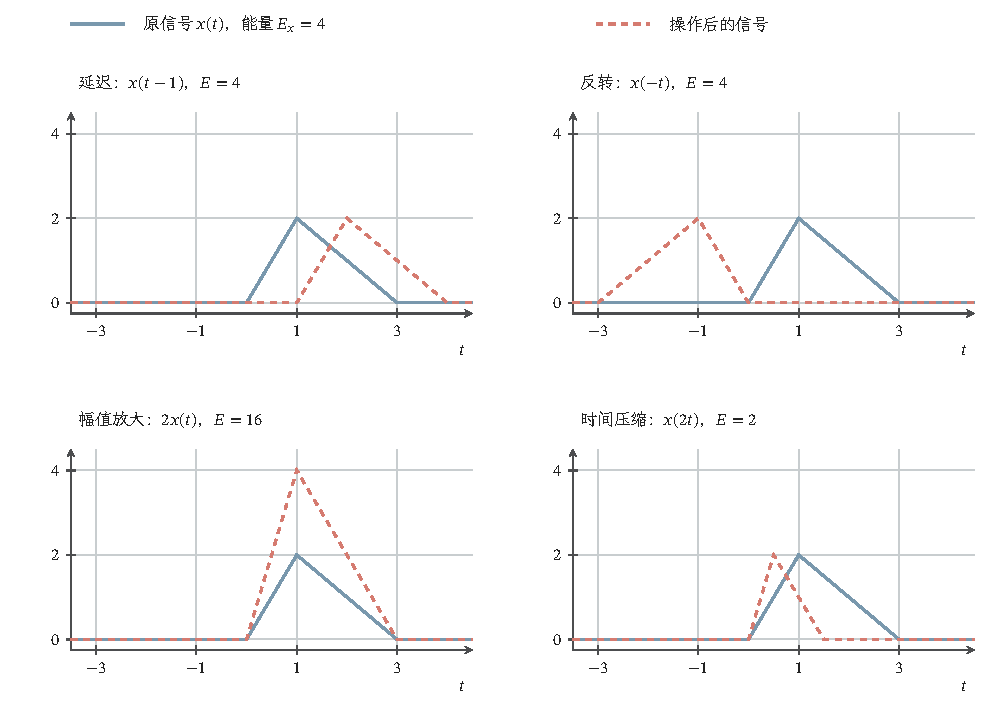
\includegraphics[width=\linewidth]{figures/01-mathematical-preliminaries/03-graphs-and-signals/tikz/signals/basic-operations.pdf}
  \caption{对同一非对称三角脉冲分别延迟、反转、放大幅值和压缩时间。
  每幅图的蓝线均为式~\eqref{eq:signal-asymmetric-wave}的原信号，红线为指定操作结果，
  横轴为时间、纵轴为幅值，坐标尺度一致。平移和反转保持整轴能量$4$，幅值乘$2$使能量变为$16$，
  时间压缩为一半使能量变为$2$；各图均在整轴零值背景下观察，不作窗口裁剪。}
  \label{fig:signal-basic-operations}
\end{figure*}

\subsection{信号的输入输出映射}
\label{sec:signal-input-output-maps}
\label{sec:signal-analysis-discrete-filtering}

一个系统是把输入信号映为输出信号的规则$y=\mathcal Hx$。
在有限位置上，线性规则可写成$y[n]=\sum_r K[n,r]x[r]$，
其中$K[n,r]$说明位置$r$的单位输入怎样影响位置$n$的输出。
整轴表达还需收敛条件，不能仅凭这个形式就交换无穷求和。
若输入、输出有$d_{\mathrm{in}}$和$d_{\mathrm{out}}$个通道，
则$K[n,r]$应为$d_{\mathrm{out}}\times d_{\mathrm{in}}$矩阵，
矩阵乘法负责混合通道，求和负责汇总时间位置，两者职责不同。

这里的因果性只表示“不读取未来输入”：若两条输入在所有$r\leq n$的位置相同，
则它们在时刻$n$的输出必须相同。对可用脉冲逐项检验的线性核映射，
这等价于$K[n,r]=0$在$r>n$时成立。
它不是第~\ref{chap:causal-inference}章用干预定义的因果响应；
只按过去顺序计算一个预测量，不会自动证明其统计关系具有干预含义。

\subsubsection{线性时不变条件下的卷积映射}
\label{sec:signal-analysis-lti-convolution}

如果改变输入幅值可以按比例叠加，而且同一个局部输入移到哪里都触发同形响应，
就有希望只保存一条响应核。两项要求需要分别定义。
\begin{definition}[线性时不变系统]
  \label{def:signal-analysis-lti-system}
  设输入、输出信号类为平移封闭的向量空间。若对任意标量$a,b$及输入$x,z$有
  $\mathcal H(ax+bz)=a\mathcal Hx+b\mathcal Hz$，称$\mathcal H$线性。
  若对每个整数$r$有
  \[
    \mathcal H(T_rx)=T_r(\mathcal Hx),
  \]
  称其具有\term{平移不变性}（shift invariance）。
  同时满足两者的系统称为线性时不变系统（linear time-invariant system, LTI）。
\end{definition}
这里输入整体移动后输出同样移动，并不是输出保持在原位置。
逐点平方$\mathcal Hx[n]=x[n]^2$平移不变却不线性，
位置加权$\mathcal Hx[n]=n\,x[n]$线性却不平移不变。
是否在每个位置调用了同一段程序，不足以替代这两项等式。

令$h=\mathcal H\delta$，称为\term{脉冲响应}（impulse response）。
有限支撑输入可按式~\eqref{eq:signal-analysis-impulse-expansion}作有限展开，
线性性与平移不变性给出
\begin{align}
  (\mathcal Hx)[n]
  &=\mathcal H\left(\sum_r x[r]T_r\delta\right)[n]\notag\\
  &=\sum_r x[r](T_rh)[n]=\sum_r x[r]h[n-r].
  \label{eq:signal-analysis-lti-convolution}
\end{align}
它把各位置输入所触发的响应相加。
对$x\in\ell_1(\mathbb Z)$，还需
$\mathcal H:\ell_1\to\ell_1$为有界线性且平移不变的算子，
即存在常数$C$使$\|\mathcal Hx\|_1\leq C\|x\|_1$。
令$x^{(K)}=\sum_{|r|\leq K}x[r]T_r\delta$，则$x^{(K)}\to x$于$\ell_1$，
有界性使$\mathcal Hx^{(K)}\to\mathcal Hx$。同时$h=\mathcal H\delta\in\ell_1$，
且
\[
  \sum_n\sum_r|x[r]h[n-r]|=\|x\|_1\|h\|_1<\infty.
\]
因此卷积和绝对收敛，有限截断的卷积也在$\ell_1$中趋于该和，
从而式~\eqref{eq:signal-analysis-lti-convolution}延伸到全部$\ell_1$输入。
不能省略连续性，直接把仅对有限和成立的代数线性搬进无穷和。

这种求和称为\term{离散卷积}（discrete convolution），规则网格上也可用同一结构。
\begin{definition}[网格上的离散卷积]
  \label{def:signal-analysis-discrete-convolution}
  对$x,h\in\ell_1(\mathbb Z^d)$，定义
  \begin{equation}
    (x*h)[\bm n]=\sum_{\bm r\in\mathbb Z^d}x[\bm r]h[\bm n-\bm r].
    \label{eq:signal-analysis-discrete-multidimensional-convolution}
  \end{equation}
  这里$\bm n,\bm r$为网格位置，$h$称为\term{卷积核}（convolution kernel）。
  各位置的和绝对收敛，输出仍属于$\ell_1(\mathbb Z^d)$。
\end{definition}
存在性可直接检查：对非负项换序并令$\bm s=\bm n-\bm r$，有
\[
  \sum_{\bm n}\sum_{\bm r}|x[\bm r]h[\bm n-\bm r]|
  =\left(\sum_{\bm r}|x[\bm r]|\right)
   \left(\sum_{\bm s}|h[\bm s]|\right)<\infty.
\]
所以每个内层和均有限，并得到
$\|x*h\|_1\leq\|x\|_1\|h\|_1$。
核为有限支撑时，对任何逐点有限的输入也可作有限和，但输出不因此必属$\ell_1$。
一维记法为
\begin{equation}
  (x*h)[n]=\sum_{r\in\mathbb Z}x[r]h[n-r].
  \label{eq:signal-analysis-linear-convolution}
\end{equation}
固定$n$后，$r$增加时核索引$n-r$减小，这就是核的反向读取。
令$s=n-r$可得$(x*h)[n]=\sum_s h[s]x[n-s]=(h*x)[n]$，故有交换律；
绝对可和等允许换序的条件还给出结合律和分配律。
若$h[r]=0$对所有$r<0$成立，则$y[n]=\sum_r h[r]x[n-r]$只用当前及过去输入，
系统因果；一般LTI则不必因果，例如三点中心均值会使用$x[n+1]$。

连续输入的局部贡献改用积分累计。
\begin{definition}[连续卷积]
  \label{def:signal-analysis-continuous-convolution}
  设$f,g\in L^1(\mathbb R^d)$，定义
  \begin{equation}
    (f*g)(\bm t)=\int_{\mathbb R^d}f(\bm\tau)g(\bm t-\bm\tau)\,\mathrm d\bm\tau.
    \label{eq:signal-analysis-continuous-convolution}
  \end{equation}
  积分对几乎处处的$\bm t$绝对收敛，并定义$L^1(\mathbb R^d)$中的元素。
\end{definition}
由定理~\ref{thm:analysis-tonelli-fubini}，对非负函数换序并平移换元，
\[
  \int_{\mathbb R^d}\int_{\mathbb R^d}
  |f(\bm\tau)g(\bm t-\bm\tau)|\,\mathrm d\bm\tau\,\mathrm d\bm t
  =\|f\|_{L^1}\|g\|_{L^1}<\infty.
\]
内层积分因而几乎处处有限，且$\|f*g\|_{L^1}\leq\|f\|_{L^1}\|g\|_{L^1}$。
换元和换序同样给出交换律、结合律，但$L^1$假设不保证每个指定点的积分都有限。
这里定义的是两个普通可积函数的卷积，并非所有连续LTI算子都具有普通$L^1$核。
例如恒等映射是LTI，它的单位脉冲响应可用Dirac分布（Dirac distribution）
$\delta_0$描述。这里“分布”采用广义函数的用语：这个对象作用于光滑紧支撑的
测试函数$\phi$时返回$\delta_0(\phi)=\phi(0)$，也就是零点单位质量对$\phi$的积分。
对这样的$f$，卷积让它读取$\tau\mapsto f(t-\tau)$在零点的值，
于是$(f*\delta_0)(t)=f(t)$，正好实现恒等映射。
普通函数$\mathbb I_{\{0\}}$的Lebesgue积分却为零，不能承担这种单位质量，
所以不能把离散$\delta[k]$直接当作连续可积核。
当前不调用一般分布理论来证明所有连续系统的核表示。

\begin{example}[区间重叠产生三角形响应]
  \label{ex:signal-analysis-continuous-overlap}
  取$f(t)=g(t)=\mathbb I_{[0,1]}(t)$。两因子同时为$1$要求
  $\tau\in[0,1]\cap[t-1,t]$，因此
  \[
    (f*g)(t)=
    \begin{cases}
      t,&0\leq t\leq1,\\
      2-t,&1<t\leq2,\\
      0,&\text{其余位置}.
    \end{cases}
  \]
  输出先随重叠长度增大而上升，再随重叠减小而下降。
  二维指示函数的相应积分计算重叠面积，一般带符号核则计算加权贡献，
  不能都解释为几何大小。
\end{example}
图~\ref{fig:reader-continuous-convolution-overlap}区分输出位置$t$和积分变量$\tau$。
三角形输出不是把两个输入图形相加，而是把每个$t$处的重叠长度汇成曲线。
\begin{figure*}[htbp]
  \centering
  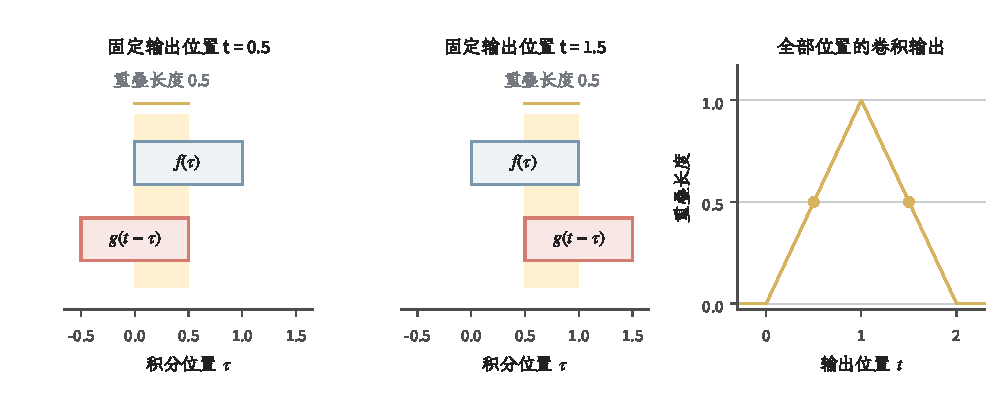
\includegraphics[width=\linewidth]{figures/01-mathematical-preliminaries/03-graphs-and-signals/matplotlib/teaching-dynamics/continuous-convolution-overlap.pdf}
  \caption{教学函数$f=g=\mathbb I_{[0,1]}$的连续卷积。左两图分别固定$t=0.5$与$t=1.5$，
  蓝色为$f(\tau)$的支撑，红色为$g(t-\tau)$的支撑，黄色重叠长度均为$0.5$。
  右图汇总全部$t$处的重叠长度，在$t=1$时达到$1$。
  左图横轴$\tau$用于积分，右图横轴$t$标记输出位置。}
  \label{fig:reader-continuous-convolution-overlap}
\end{figure*}

回到有限输入。若$x,h$的支撑分别为$0,\ldots,m-1$和$0,\ldots,r-1$，
零延拓线性卷积只可能在$0,\ldots,m+r-2$非零，完整输出长度为$m+r-1$。
贯穿例逐项为
\begin{align*}
  (x*h)[0]&=1,\\
  (x*h)[1]&=2-1=1,\\
  (x*h)[2]&=1-2=-1,\\
  (x*h)[3]&=-1.
\end{align*}
即
\begin{equation}
  \bm x*\bm h=(1,1,-1,-1).
  \label{eq:signal-analysis-running-linear-convolution}
\end{equation}
这个核计算当前值减去前一个值，首尾还包含零延拓带来的跳变。
长度$N$的循环索引则在一个周期内求和：
\begin{equation}
  (x*_Nh)[n]=\sum_{r=0}^{N-1}x[r]h[(n-r)\bmod N],
  \qquad n=0,\ldots,N-1.
  \label{eq:signal-analysis-circular-convolution}
\end{equation}
\begin{definition}[循环卷积]
  \label{def:signal-analysis-circular-convolution}
  对长度$N$的实或复序列，式~\eqref{eq:signal-analysis-circular-convolution}
  定义其\term{循环卷积}（circular convolution），输出仍有$N$项。
  它在有限循环索引集上求和，不是两条周期延拓序列在整数轴上的无穷卷积。
\end{definition}
把$h$补成$(1,-1,0)$并取$N=3$，得到$x*_3h=(0,1,-1)$。
完整线性卷积的末项$-1$回绕到首项，与$1$相消；不是直接删掉了末项。
若对两条周期序列在整轴无穷求和，同一贡献会被重复无穷次。
图~\ref{fig:signal-convolution-boundaries}对比零延拓与循环边界下的输出。
\begin{figure}[!htb]
  \centering
  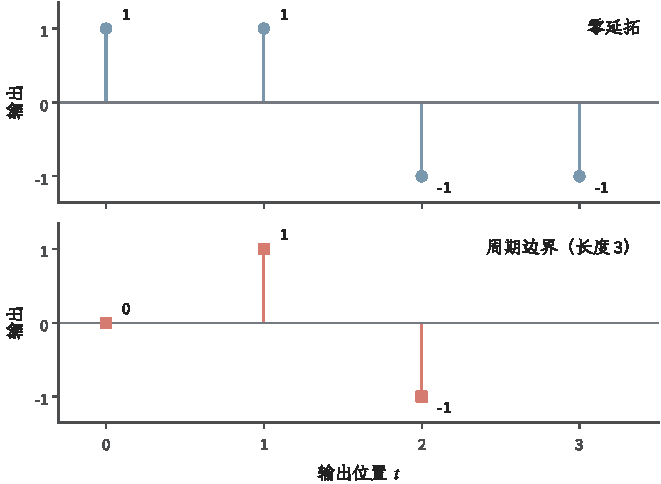
\includegraphics[width=\linewidth]{figures/01-mathematical-preliminaries/03-graphs-and-signals/matplotlib/dynamics/convolution-boundaries.pdf}
  \caption{输入$(1,2,1)$与核$(1,-1)$的边界比较。蓝色圆点采用零延拓，给出四项线性卷积；
  红色方点采用长度$3$的循环边界，末项$-1$回到首项并与$1$抵消。
  连线只指示离散数值的顺序，不定义整数之间的信号值。}
  \label{fig:signal-convolution-boundaries}
\end{figure}

固定输入输出位置后，线性卷积是Toeplitz矩阵乘法，循环卷积是循环矩阵乘法。
例如同一个贯穿例给出
\begin{gather*}
  \begin{bmatrix}
    1&0&0\\-1&1&0\\0&-1&1\\0&0&-1
  \end{bmatrix}
  \begin{bmatrix}1\\2\\1\end{bmatrix}
  =\begin{bmatrix}1\\1\\-1\\-1\end{bmatrix},\\
  \begin{bmatrix}1&0&-1\\-1&1&0\\0&-1&1\end{bmatrix}
  \begin{bmatrix}1\\2\\1\end{bmatrix}
  =\begin{bmatrix}0\\1\\-1\end{bmatrix}.
\end{gather*}
重复对角线反映参数共享，边界则改变矩阵首尾行。
无限网格或循环群上的平移不变性是精确的；有限区间采用零填充、反射或截取后，
通常不再具有同一意义的全局平移不变性。

“valid”只选择核完全落在已知输入内的输出。
按$h[0],\ldots,h[r-1]$的因果索引，当$m\geq r$时保留$n=r-1,\ldots,m-1$，
共$m-r+1$项；$m<r$时没有这样的输出。
保持输入长度的“same”还需指定左右填充及截取位置，不能只凭名称确定。
表~\ref{tab:signal-boundary-conventions}将延拓和输出选择分开，
后文FFT也必须遵守同一约定。
\begin{table*}[!htb]
  \centering
  \begin{tabularx}{\linewidth}{lXXX}
    \toprule
    约定 & 区间外输入 & 保留输出 & 贯穿例\\
    \midrule
    完整线性卷积 & 零延拓 & $0,\ldots,m+r-2$ & $(1,1,-1,-1)$\\
    有效区间选段 & 不使用区间外值 & $r-1,\ldots,m-1$，$m\geq r$ & $(1,-1)$\\
    $N$点循环卷积 & 周期边界 & $0,\ldots,N-1$ & $N=3$时$(0,1,-1)$\\
    \bottomrule
  \end{tabularx}
  \caption{边界延拓与输出选段。$m$为输入长度，$r$为核长度，使用本章因果核索引。
  有效选段不是另一种卷积定义，循环边界也不是零边界的近似。}
  \label{tab:signal-boundary-conventions}
\end{table*}

有了有限DFT，循环卷积可在频率坐标中逐项计算。
\begin{theorem}[离散循环卷积定理]
  \label{thm:signal-analysis-circular-convolution-theorem}
  设$x,h$为长度$N$的复序列，采用式~\eqref{eq:signal-analysis-dft}的约定，则
  \[
    \widehat{x*_Nh}[k]=\widehat x[k]\widehat h[k],\qquad k=0,\ldots,N-1.
  \]
\end{theorem}
\begin{proof}
  令$a=(n-r)\bmod N$，直接换有限求和的索引，
  \begin{align*}
    \widehat{x*_Nh}[k]
    &=\sum_{n=0}^{N-1}\sum_{r=0}^{N-1}
      x[r]h[(n-r)\bmod N]\omega_N^{kn}\\
    &=\sum_{r=0}^{N-1}\sum_{a=0}^{N-1}
      x[r]h[a]\omega_N^{k(r+a)}\\
    &=\left(\sum_{r=0}^{N-1}x[r]\omega_N^{kr}\right)
      \left(\sum_{a=0}^{N-1}h[a]\omega_N^{ka}\right).
  \end{align*}
  固定$r$后，$n$遍历一个周期使$a$也恰遍历一个周期。
  即使$n$与$r+a$相差$N$的整数倍，$\omega_N^{kN}=1$仍使指数相同。
  最后两项分别为$\widehat x[k]$与$\widehat h[k]$。
\end{proof}
于是
\begin{equation}
  x*_Nh=\mathcal F_N^{-1}\bigl(\mathcal F_N(x)\odot\mathcal F_N(h)\bigr).
  \label{eq:signal-analysis-frequency-domain-convolution}
\end{equation}
若$\bm C_h$为循环卷积矩阵，定理对所有$x$成立，故
$\bm F\bm C_h=\operatorname{diag}(\widehat{\bm h})\bm F$，从而
$\bm C_h=\bm F^{-1}\operatorname{diag}(\widehat{\bm h})\bm F$。
这完整说明DFT如何对角化循环卷积：核的DFT系数是各频率模式的特征值。
要用它得到完整线性卷积，两个输入均须补零到
\begin{equation}
  N\geq m+r-1.
  \label{eq:signal-analysis-linear-padding-condition}
\end{equation}
因为所有非零输出索引此时都小于$N$，不会回绕。
$N\geq\max(m,r)$只保证装下输入，不保证装下输出。

整轴频率响应改用DTFT。若$h\in\ell_1$或具有有限支撑，
即使复指数$x[n]=e^{\mathrm i\omega n}$自身不在$\ell_1$中，仍有绝对收敛的和
\[
  (x*h)[n]=\sum_r h[r]e^{\mathrm i\omega(n-r)}
  =e^{\mathrm i\omega n}\sum_r h[r]e^{-\mathrm i\omega r}.
\]
输出保持频率，只乘以
\begin{equation}
  H(e^{\mathrm i\omega})=\sum_r h[r]e^{-\mathrm i\omega r},
  \label{eq:signal-analysis-filter-frequency-response}
\end{equation}
即\term{频率响应}（frequency response）。模长给出放大或衰减，相角给出该模式的
相位变化；除非相位随频率具有相应线性形式，不能将所有频率的相位变化都叫同一时间延迟。
对$x,h\in\ell_1$，绝对可和允许换序，直接得到
$Y(e^{\mathrm i\omega})=X(e^{\mathrm i\omega})H(e^{\mathrm i\omega})$。
同理，连续$L^1$卷积的傅里叶变换为$F(\Omega)G(\Omega)$，
其积分换序由前面的绝对积分界保证。

贯穿核的响应为$H(e^{\mathrm i\omega})=1-e^{-\mathrm i\omega}$，
模长为$2|\sin(\omega/2)|$。常量模式$\omega=0$被消去，低频缓变被削弱，
较高频的差异更突出；这解释了它为何是一阶差分，而有限输入首尾仍受延拓影响。

多通道卷积将标量核换成矩阵核：
\begin{equation}
  y_a[n]=\sum_{b=1}^{d_{\mathrm{in}}}\sum_{r\in\mathbb Z}
  H_{a,b}[r]x_b[n-r],
  \qquad a=1,\ldots,d_{\mathrm{out}}.
  \label{eq:signal-multichannel-convolution}
\end{equation}
各$H_{a,b}\in\ell_1$、各$x_b\in\ell_1$时，有限通道求和与前述界保证存在性；
有限核则在每个位置作有限计算。相同输入输出通道数且$\bm H[r]$总是对角矩阵时，
各通道独立滤波；非对角元素允许输入通道$b$影响输出通道$a$。
频域关系相应为$\widehat{\bm y}[k]=\widehat{\bm H}[k]\widehat{\bm x}[k]$，
每个频率上是矩阵乘向量，不是把所有通道分别做一个标量乘法。

无时间记忆的特例$\bm H[0]=\bm B$、其余为零，只在同一时刻混合通道。
取式~\eqref{eq:signal-multichannel-record}中的记录及
$\bm B=\begin{bmatrix}1&1\\1&-1\end{bmatrix}$，有
\[
  \bm Y=\bm X\bm B^\top
  =\begin{bmatrix}1&1\\3&1\\3&-1\end{bmatrix}.
\]
如图~\ref{fig:signal-channel-mixing}所示，输出第一通道为和，第二通道为差，
三个时间位置未变。总能量从$11$变为$22$，因为$\bm B^\top\bm B=2\bm I$；
用$\bm B/\sqrt2$才保持能量。混合前若两路未按时间对齐，矩阵计算本身不会修正偏移。
\begin{figure*}[htbp]
  \centering
  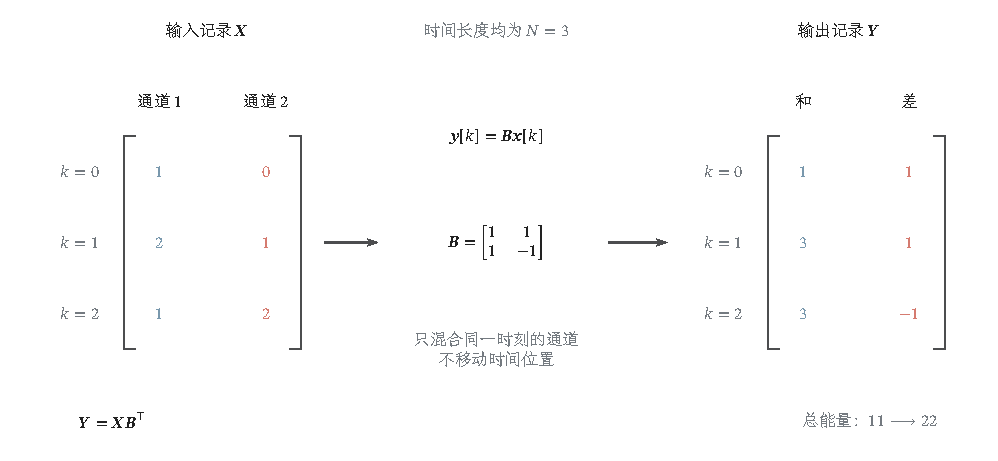
\includegraphics[width=\linewidth]{figures/01-mathematical-preliminaries/03-graphs-and-signals/tikz/signals/channel-mixing.pdf}
  \caption{同一双通道三时刻记录的轴与混合。左侧行标记时间、列标记通道；
  中间矩阵$\bm B$对每一行对应的同时读数取和与差，右侧时间轴长度仍为$3$。
  通道混合不是时间平移，也不意味着两个输入通道独立；这里只使用当前时刻的值。}
  \label{fig:signal-channel-mixing}
\end{figure*}

\subsubsection{线性时变条件下的历史映射}

设备增益随时刻变化时，同样的脉冲在不同时间可能触发不同响应，线性却仍可成立。
用已给定的两时刻核表示
\begin{equation}
  \bm y[n]=\sum_{r\leq n}\bm K[n,r]\bm x[r].
  \label{eq:signal-given-time-varying-kernel}
\end{equation}
有限历史窗口中它是有限和；无限历史中则需另行保证收敛，
例如对有界输入可要求$\sum_{r\leq n}\|\bm K[n,r]\|<\infty$。
求和只取$r\leq n$规定因果性，矩阵维度仍为
$d_{\mathrm{out}}\times d_{\mathrm{in}}$。
核事先固定、不随输入改变时，该表达满足叠加。
若同时满足$\bm K[n+s,r+s]=\bm K[n,r]$，才只依赖滞后$n-r$，
并可记成固定卷积核；只因它累加历史，不能省掉这项条件。

例如令$a[n]$在偶数时为$1$、奇数时为$2$，
$y[n]=a[n](x[n]+\tfrac12x[n-1])$。
它的两时刻核仅在$r=n,n-1$非零，且取值随绝对时刻$n$变化。
输入$\delta[n]$在时刻$0$给出$1$，将输入延迟一格后，时刻$1$的输出却为$2$，
而原输出延迟一格在该处仍为$1$，因此不平移不变。
相反，事先给定$h[0]=0$、$h[r]=2^{-(r-1)}$（$r\geq1$）及负索引为零，
就定义了一个有衰减记忆的固定卷积核。对零延拓$x=(1,2,1)$，
从时刻$0$起的前四项输出为$(0,1,5/2,9/4)$，每次使用相同的滞后权重。

这些例子只需知道输入输出核，不需先引入内部状态。
第~\ref{sec:signal-analysis-state-history-kernels}节将从状态演化构造固定核与两时刻核，
并区分初始状态的自由响应、直接项和输入驱动项。
那里的有序矩阵乘积解释核从何而来；本节检验的是给定核定义了什么映射。
若另加一个与输入无关且非零的自由响应，总映射一般是仿射而非线性，
不能仅因输入驱动部分线性就忽略这一差别。

\subsubsection{非线性条件下的输入依赖映射}

核如果根据当前输入调整，冻结核后的一次矩阵乘法也不能代表整个映射。
最简单的例子是$(\mathcal Hx)[n]=x[n]^2$：对$x[n]=1$，
$\mathcal H(2x)[n]=4\neq2\mathcal Hx[n]$，故不线性。
但$\mathcal H(T_rx)[n]=x[n-r]^2=T_r(\mathcal Hx)[n]$，所以它仍平移不变，
且只使用当前值，满足这里的因果性。

再看输入依赖门控
\[
  y[n]=g(x[n])x[n],\qquad g(v)=\frac1{1+e^{-v}}
\]
（此例取实数输入）。门控是由当前输入决定的权重。
输入$1$与$2$得到的比例分别是$g(1)$与$g(2)$，两者不同，
所以$y(2)\neq2y(1)$；尽管每个位置使用同一规则，叠加仍不成立。
更一般的$\sum_{r\leq n}K_x[n,r]x[r]$既要检查核如何依赖输入，
也要检查计算$K_x$时是否偷用了未来值。求和表面上只到$n$，
不代表输入依赖的权重一定因果。

可微映射在固定输入附近可以线性化。例如平方映射满足
$(x_0+\varepsilon v)^2=x_0^2+2\varepsilon x_0v+\varepsilon^2v^2$，
一阶响应是$v\mapsto2x_0v$。它依赖展开位置$x_0$，只描述小扰动；
不能据此给全部输入配同一个频率响应。
状态参数若由输入选择，也会出现同样边界，具体构造仍回查
第~\ref{sec:signal-analysis-state-history-kernels}节。

\subsection{基于相关运算的模板比较}
\label{sec:signal-template-correlation}

卷积叠加输入激起的响应；寻找某个波形出现在哪里，则更自然地把模板与不同片段作内积。
采用本章方向约定，\term{互相关}（cross-correlation）为
\begin{equation}
  (x\star h)[n]=\sum_{r\in\mathbb Z}x[n+r]\overline{h[r]}.
  \label{eq:signal-analysis-cross-correlation}
\end{equation}
固定$n$后，比较的是片段$r\mapsto x[n+r]$与原方向模板$r\mapsto h[r]$；
第二个变量取共轭，与前面的内积约定一致。
若$x,h\in\ell_2$，Cauchy--Schwarz保证每个$n$处绝对收敛；
有限模板则只需对应片段逐点有定义。

令$\widetilde h[r]=\overline{h[-r]}$，换元可得
\[
  (x*\widetilde h)[n]=\sum_s x[s]\overline{h[s-n]}
  =\sum_r x[n+r]\overline{h[r]}=(x\star h)[n].
\]
所以相关可以用共轭反转核的卷积实现，模板自身却按原方向比较。
多通道模板在同一$n$处按已声明的通道内积汇总：
$\sum_r\sum_c x_c[n+r]\overline{h_c[r]}$，
带权版本为$\sum_r\bm h[r]^*\bm W\bm x[n+r]$。
若归一化，应同时使用当前片段与模板的非零范数，窗口或权重变化也会改变相似性。

仍取零延拓$x=(1,2,1)$、$h=(1,-1)$。
模板完全在输入内时，相关在$n=0,1$得到$1-2=-1$与$2-1=1$；
完整相关在$n=-1,0,1,2$依次为$(-1,-1,1,1)$。
完整卷积则在$n=0,1,2,3$得到$(1,1,-1,-1)$，
而valid卷积在$n=1,2$给出$(1,-1)$。
差异既来自核方向，也来自输出索引，不能只看数组长度判断二者相同。
许多神经网络库把不反转实核的相关称为“卷积”，训练参数可适应该约定；
手算、复用核或推导伴随算子时，仍须明确反转、共轭、延拓及输出范围。

\subsection{卷积映射的快速计算}
\label{sec:signal-analysis-fast-transforms}

先固定所求的是完整线性卷积、循环卷积，还是某个valid输出块，再比较计算路线。
对有限序列的多项式$X(z)=\sum_{i=0}^{m-1}x_i z^i$与
$H(z)=\sum_{j=0}^{r-1}h_jz^j$，乘积为
\begin{align}
  X(z)H(z)
  &=\sum_{i=0}^{m-1}\sum_{j=0}^{r-1}x_i h_jz^{i+j}\notag\\
  &=\sum_{n=0}^{m+r-2}\left(\sum_{i+j=n}x_i h_j\right)z^n.
  \label{eq:signal-analysis-polynomial-convolution}
\end{align}
系数恰为线性卷积，多项式的交换律与结合律也解释了有限卷积的相应性质。
贯穿例给出
\begin{equation}
  P(z)=(1+2z+z^2)(1-z)=1+z-z^2-z^3.
  \label{eq:signal-analysis-running-polynomial-product}
\end{equation}
循环边界则在乘积后取余：
\begin{equation}
  (XH)\bmod(z^N-1)=\sum_{n=0}^{N-1}(x*_Nh)[n]z^n,
  \label{eq:signal-analysis-polynomial-circular-convolution}
\end{equation}
这里$x,h$均以长度$N$编码，$z^{N+s}\equiv z^s$正好合并回绕项。
乘积次数小于$N$时取模不改系数，与补零条件一致。
这些对应本身没有减少运算；收益来自利用点值或余数中的乘法结构。

\subsubsection{单位根分解下的FFT计算}

直接求$N$个DFT系数需要$O(N^2)$运算，再调用卷积定理并未自动提速。
\term{快速傅里叶变换}（fast Fourier transform, FFT）是一族快速计算DFT的算法，
不是另一种频率变换。基二Cooley--Tukey分解利用偶数长度的单位根结构复用子结果
\scite{cooley1965fft}
令$x_{\mathrm e}[r]=x[2r]$、$x_{\mathrm o}[r]=x[2r+1]$，
它们的$N/2$点DFT为$E[k],O[k]$。因为$\omega_N^2=\omega_{N/2}$，
\[
  \widehat x[k]
  =\sum_{r=0}^{N/2-1}x[2r]\omega_{N/2}^{kr}
   +\omega_N^k\sum_{r=0}^{N/2-1}x[2r+1]\omega_{N/2}^{kr}.
\]
而$\omega_N^{N/2}=-1$，子变换以$N/2$为周期，所以对$0\leq k<N/2$有蝶形关系
\begin{align}
  \widehat x[k]&=E[k]+\omega_N^kO[k],\notag\\
  \widehat x[k+N/2]&=E[k]-\omega_N^kO[k].
  \label{eq:signal-analysis-fft-butterfly}
\end{align}
同一对中间结果产生两个频率，没有舍弃后一半。
当$N=2^q$时，$T(N)=2T(N/2)+O(N)$，共$q$层、每层$O(N)$运算，
所以复杂度为$O(N\log N)$。
其他合数长度可按其他因子分解，质数长度也有相应算法；
补到二的幂只是某些实现的便利选择，不是FFT的普遍必要条件。

贯穿例补零到$N=4$，取$\bm x_4=(1,2,1,0)$、$\bm h_4=(1,-1,0,0)$。
$x_4$的偶分支$(1,1)$的二点DFT为$(2,0)$，奇分支$(2,0)$的为$(2,2)$。
用$\omega_4=-\mathrm i$合并得到
\[
  \widehat{\bm x}_4=(2+2,\ 0-2\mathrm i,\ 2-2,\ 0+2\mathrm i)
  =(4,-2\mathrm i,0,2\mathrm i).
\]
$h_4$的偶、奇分支DFT分别为$(1,1)$与$(-1,-1)$，同样得到
$\widehat{\bm h}_4=(0,1+\mathrm i,2,1-\mathrm i)$。
这一步显示如何复用两个二点变换，而不只是代入四点定义。
对$x_4$逆变换的四个分子依次为
\[
  4-2\mathrm i+2\mathrm i,\quad 4+2+2,\quad
  4+2\mathrm i-2\mathrm i,\quad 4-2-2,
\]
除以$4$后恢复$(1,2,1,0)$，同时核对了频率顺序、指数符号及归一化。
逐点乘积
$\widehat{\bm x}_4\odot\widehat{\bm h}_4=(0,2-2\mathrm i,0,2+2\mathrm i)$，
逆DFT给出$(1,1,-1,-1)$。若只用$N=3$，得到的是$(0,1,-1)$，
因为末项已经回绕；再精确的FFT也不能把这个循环输出当作原完整卷积。

\subsubsection{一般选点下的Toom–Cook计算}

单位根方便递归，但乘积恢复并不只允许这种选点。
Toom--Cook方法对多项式分块、求值、逐点相乘，再插值恢复系数。
对二次$X$与一次$H$，乘积次数至多为$3$，
可使用$0,1,-1,\infty$四个坐标；其中“无穷点”表示读取最高次系数，
不是把无穷大传给数值程序\scite{math-knuth1997seminumerical}
记
\begin{align*}
  r_0&=X(0)H(0),&r_+&=X(1)H(1),\\
  r_-&=X(-1)H(-1),&r_\infty&=x_2h_1.
\end{align*}
设$P(z)=c_0+c_1z+c_2z^2+c_3z^3$，
则$r_+=c_0+c_1+c_2+c_3$，$r_-=c_0-c_1+c_2-c_3$，
和、差分别解出偶次与奇次部分：
\begin{align}
  c_0&=r_0,\qquad c_3=r_\infty,\notag\\
  c_1&=\frac{r_+-r_-}{2}-c_3,\notag\\
  c_2&=\frac{r_++r_-}{2}-c_0.
  \label{eq:signal-analysis-toom-reconstruction}
\end{align}
这是前述插值思想在包含最高次坐标时的具体形式；分母$2$要求系数域中$2$可逆。

贯穿例的四个值为$(r_0,r_+,r_-,r_\infty)=(1,0,0,-1)$，
恢复为$(c_0,c_1,c_2,c_3)=(1,1,-1,-1)$。
直接展开需$3\times2=6$次输入系数与核系数相乘，此方案只需四次点值乘法，
却增加了求值、插值及常数乘除。长多项式可递归分块获得渐近改进，
短核则未必值得；缓存、数据变换和访存也要计入。
点值乘法之所以成立，是因为$P(a)=X(a)H(a)$，不是因为任意坐标变换都把乘法变为逐点乘法。

\subsubsection{互素模分解下的Winograd计算}

更一般的路线在低次模下先相乘，再用中国剩余定理恢复，
因为$(XH)\bmod m$只需$X\bmod m$和$H\bmod m$。
Winograd类算法据此构造较少乘法的乘积或滤波计算，特定输出块还需相应的恢复映射
\scite{math-winograd1980arithmetic}
先对同一完整乘积取
$M(z)=z^4-1=(z-1)(z+1)(z^2+1)$。
三个实系数因子两两互素、总次数为$4$，分别有
\[
  P(1)=0,\quad P(-1)=0,\qquad
  X\bmod(z^2+1)=2z,\quad H\bmod(z^2+1)=1-z.
\]
在第三个模下$z^2=-1$，所以$XH\equiv2+2z$。
设恢复的$R$次数小于$4$，前两份零余数使
$R(z)=(z^2-1)(az+b)$。再模$z^2+1$得到$R\equiv-2az-2b$，
与$2+2z$比较便有$a=b=-1$，从而$R=1+z-z^2-z^3$。
原乘积次数已经小于$4$，因此这正是完整乘积；若次数更高，就只能得到模代表元。
本次映射从长度$3$和$2$的输入恢复四项完整卷积，不能直接称作任意输出块的最小算法。

\begin{example}[可复核的Winograd \(F(2,3)\)输出块]
  \label{ex:signal-analysis-winograd-f23}
  固定一维valid互相关，输入$\bm d=(d_0,d_1,d_2,d_3)^\top$，
  核$\bm g=(g_0,g_1,g_2)^\top$，所需输出只有
  \begin{align*}
    y_0&=d_0g_0+d_1g_1+d_2g_2,\\
    y_1&=d_1g_0+d_2g_1+d_3g_2.
  \end{align*}
  $F(2,3)$使用关于$z,z-1,z+1$的余数与最高次系数坐标。
  核侧是$0,1,-1$处点值及最高次系数的缩放；
  输入侧则针对只恢复两项输出另作线性组合。一组符合本章方向约定的变换为
  \begin{equation}
    \bm y=\bm A^\top\bigl[(\bm G\bm g)\odot(\bm B^\top\bm d)\bigr],
    \label{eq:signal-analysis-winograd-f23}
  \end{equation}
  其中
  \begin{align*}
    \bm B^\top&=\begin{bmatrix}
      1&0&-1&0\\0&1&1&0\\0&-1&1&0\\0&1&0&-1
    \end{bmatrix},\\
    \bm G&=\begin{bmatrix}
      1&0&0\\1/2&1/2&1/2\\1/2&-1/2&1/2\\0&0&1
    \end{bmatrix},\\
    \bm A^\top&=\begin{bmatrix}1&1&1&0\\0&1&-1&-1\end{bmatrix}.
  \end{align*}
  形状分别为$\mathbb R^4\to\mathbb R^4$、$\mathbb R^3\to\mathbb R^4$，
  逐点相乘后由$\mathbb R^4\to\mathbb R^2$恢复指定输出。
  为直接核对恒等式，记
  \begin{align*}
    m_0&=(d_0-d_2)g_0,\\
    m_1&=\tfrac12(d_1+d_2)(g_0+g_1+g_2),\\
    m_2&=\tfrac12(-d_1+d_2)(g_0-g_1+g_2),\\
    m_3&=(d_1-d_3)g_2.
  \end{align*}
  则$m_1+m_2=d_2g_0+d_1g_1+d_2g_2$，
  $m_1-m_2=d_1g_0+d_2g_1+d_1g_2$，
  所以$m_0+m_1+m_2=y_0$、$m_1-m_2-m_3=y_1$。

  取$\bm d=(1,2,3,4)^\top$、$\bm g=(2,-1,1)^\top$，
  有$\bm B^\top\bm d=(-2,5,1,-2)^\top$、
  $\bm G\bm g=(2,1,2,1)^\top$。四次逐点相乘得到
  $\bm m=(-4,5,2,-2)^\top$，输出变换给出$(3,5)^\top$。
  直接互相关也有$2-2+3=3$、$4-3+4=5$。
  六次输入--核乘法减少为四次，但变换的加减和常数运算仍有成本。
\end{example}

三条路线共同利用乘法兼容的表示，结构却不同。
FFT在$z^N-1$的全部复单位根处求值，并利用根的规则结构快速变换；
Toom--Cook允许一般选点及递归分块；Winograd类构造用互素余数并常针对指定小块输出。
一次因子的CRT与点值插值重合，高次因子保留的却是一个低次多项式，不能称为单个点值。

长度相近的两个$n$项序列直接卷积需要$O(n^2)$次乘加，
FFT路线在合适长度上需$O(N\log N)$变换运算及$N$次频域乘法。
乘法数和渐近量级并非完整运行时间：加减、复数算术、常数运算、缓存复用与目标硬件
都会改变实际排序。归一化DFT是酉变换、条件良好，但多层蝶形仍会累积舍入误差；
Toom--Cook和Winograd的变换矩阵可能有较大尺度差异，相近量相减也会放大相对误差。

整数或有限域算法还要检查系数域条件。一个有限域（finite field）的例子是
模素数$p$的数系：只保留$0,\ldots,p-1$，加乘后取模，非零元素都有乘法逆元。
例如模$5$时$2\cdot3=1$，所以除以$2$就是乘以$3$。
数论变换（number-theoretic transform, NTT）在这类数系中按DFT的形式求值；
它需要所需阶数的单位根，逆变换中的$N$也须可逆。
若$p$整除$N$，$N$在该数系中就是零，不能作为除数；
前面Toom--Cook的除以$2$也有同样的系数域限制。

若目标是恢复整数系数，还要从有限域运算返回整数余数重构。
此处的模数是整数，与前面的模多项式不同。设总整数模数为$Q$
（使用多个两两互素模数时取它们的乘积），选取区间$(-Q/2,Q/2]$内的余数代表。
已知每个真实系数绝对值不超过$B$时，$Q>2B$保证该代表唯一等于真实系数：
两个候选系数之差绝对值至多$2B$，不可能是非零的$Q$倍数。
第$n$个卷积系数的绝对值可由$\sum_{i+j=n}|x_i h_j|$控制，
再对输出位置取统一上界即可选取$B$。
避免浮点误差并不等于避免模混淆或整数溢出。
没有脱离规模、数据类型和误差目标的普遍最优算法。

最后仍需返回目标映射：FFT线性卷积要满足补零条件，Toom--Cook恢复所设多项式乘积，
网络互相关要另行核对核方向；Winograd只恢复设计的输出块，
步长、空洞率或边界变动后要重新推导。提速改变求值顺序，不增加信息，也不替用户选择边界。

\section{信号的采样与恢复}
\label{sec:signal-analysis-sampling}

完整DFT能恢复输入数组，却不能据此恢复产生数组的任意连续信号。
采样只读取一些位置，可能把不同信号映为相同数据；重构必须靠额外的信号类约束
排除这种歧义。本节先说明何种区别在采样时消失，再给出带限条件下的恢复定理，
最后区分精确恢复与采样前主动改变频率内容的预滤波。

\subsection{采样映射与混叠歧义}
\label{sec:signal-sampling-ambiguity}

固定时间原点及采样间隔$T_s>0$，对具有确定点值的连续时间信号$f$读取
$x[n]=f(nT_s)$，采样频率为$\nu_s=1/T_s$。
若不约束候选信号，采样通常不是单射。
例如$T_s=1$时，$f_1(t)=\cos(0.8\pi t)$与$f_2(t)=\cos(1.2\pi t)$频率不同，
却满足
\[
  f_2(n)=\cos(2\pi n-0.8\pi n)=\cos(0.8\pi n)=f_1(n),
  \qquad n\in\mathbb Z.
\]
这是\term{混叠}（aliasing）：不同连续振荡在样本上无法区分。
图~\ref{fig:signal-aliasing-curves}中的两条曲线在样本之间起伏不同，
但每个整数位置都穿过同一点。
\begin{figure}[htbp]
  \centering
  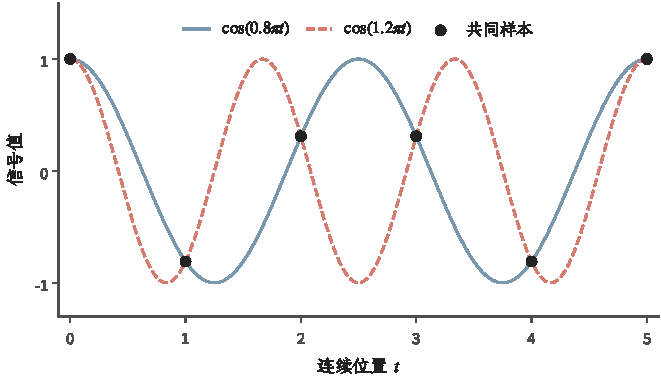
\includegraphics[width=\linewidth]{figures/01-mathematical-preliminaries/03-graphs-and-signals/matplotlib/dynamics/aliasing-curves.pdf}
  \caption{教学构造$f_1(t)=\cos(0.8\pi t)$与$f_2(t)=\cos(1.2\pi t)$。
  蓝色实线和红色虚线在整数时刻具有共同样本，深灰圆点标出这些观测。
  图只展示$[0,5]$，样本相同对所有整数成立；两条纯余弦是功率信号，
  不属于后文定理中的整轴平方可积信号类。}
  \label{fig:signal-aliasing-curves}
\end{figure}

任何确定性插值器对相同输入样本只能返回同一输出，因此不可能同时正确恢复这两条曲线。
学习模型可以凭训练分布猜测更常见的细节，但这种能力来自额外先验，
不是采样映射自己变成可逆。这里的余弦有有限平均功率而整轴能量无穷，
只用于展示歧义；后文将换到$L^2$带限空间，不能把此例当作那个空间中的反例。
对一般$L^2$等价类，点值采样本身还未定义，下一小节会先补齐代表元条件。

离散信号也可以丢弃位置。对正整数$M$保留每$M$项中的一项，
$y[n]=x[Mn]$，称为$M$倍\term{下采样}（downsampling）。
其DTFT满足
\begin{equation}
  Y(e^{\mathrm i\omega})=\frac1M\sum_{\ell=0}^{M-1}
  X\left(e^{\mathrm i(\omega+2\pi\ell)/M}\right).
  \label{eq:signal-analysis-downsampling-spectrum}
\end{equation}
对$x\in\ell_1$，按定义展开右侧并交换有限和与绝对收敛级数，
\begin{align*}
  \frac1M\sum_{\ell=0}^{M-1}X\left(e^{\mathrm i(\omega+2\pi\ell)/M}\right)
  &=\sum_{r\in\mathbb Z}x[r]e^{-\mathrm ir\omega/M}
    \left(\frac1M\sum_{\ell=0}^{M-1}e^{-2\pi\mathrm i\ell r/M}\right)\\
  &=\sum_{n\in\mathbb Z}x[Mn]e^{-\mathrm i\omega n}.
\end{align*}
括号内的单位根和只在$M\mid r$时为$1$，否则为$0$，故留下的恰为输出DTFT。
对$x\in\ell_2$，下采样满足$\sum_n|x[Mn]|^2\leq\sum_r|x[r]|^2$，
频域右侧的有限分支映射在$L^2$中也有界；
先对有限截断证明再取$L^2$极限，便得到同一公式的等价类解释。

输入模式$e^{\mathrm i\omega_0n}$变为$e^{\mathrm iM\omega_0n}$，
输入频率映到$M\omega_0\bmod2\pi$。
原频谱沿输出频率轴扩展$M$倍，超出主值区间的部分回绕，与其他分量相加。
所以“样本点变少”不只是频率曲线画得稀疏，而可能直接合并原来不同的频率。
连续采样的频谱复制也有类似现象，但必须在可读取点值的信号类上推导。

\subsection{信号约束下的恢复与预滤波}

排除歧义有两种不同做法：限制原信号本来就属于可恢复的类，或者先改变原信号，
使准备保留的部分适合新的采样间隔。前者讨论从原信号样本精确恢复，
后者讨论采样前删掉或压低哪些分量，恢复目标也随之改变。

\subsubsection{带限条件下的精确恢复}
\label{sec:signal-bandlimited-recovery}

带限用频率约束限制候选函数，而非只规定观察多长时间。
\begin{definition}[平方可积带限信号]
  \label{def:signal-analysis-bandlimited-space}
  设$\Omega_{\max}>0$、$f\in L^2(\mathbb R)$，其Plancherel意义的傅里叶变换为$F$。
  若$F(\Omega)=0$对几乎处处的$|\Omega|>\Omega_{\max}$成立，
  称$f$带限于$\Omega_{\max}$。
  所有这类函数组成\term{Paley--Wiener带限空间}。
\end{definition}
只观察一个有限时间窗口，不能推出窗口外为零，更不能推出高频为零。
带限才是下面用来排除混叠的信号类条件。

带限还使点值有规范含义。由$F\in L^2$及频谱支撑长度有限，
Cauchy--Schwarz不等式给出
\[
  \|F\|_1\leq\sqrt{2\Omega_{\max}}\,\|F\|_2<\infty.
\]
因此
\[
  f_{\mathrm c}(t)=\frac1{2\pi}\int_{-\Omega_{\max}}^{\Omega_{\max}}
  F(\Omega)e^{\mathrm i\Omega t}\,\mathrm d\Omega
\]
是$f$的连续代表元；连续性由以$|F|$为可积控制函数的控制收敛得到。
两个连续代表元若几乎处处相等，就处处相等，所以这种选择唯一。
以下仍记它为$f$，样本$f(nT_s)$都针对这个代表元，不针对随意改过点值的版本。

记采样角频率$\Omega_s=2\pi/T_s$，基带
$I_s=[-\pi/T_s,\pi/T_s]$。这里\term{基带}（baseband）指选定的一段基本频率区间。
将频谱副本按间隔$\Omega_s$相加，
\[
  P_F(\Omega)=\frac1{T_s}\sum_{k\in\mathbb Z}F(\Omega-k\Omega_s).
\]
由于$F$带限，在$I_s$上只有有限多个平移副本可能非零，故$P_F\in L^2(I_s)$，
并以$\Omega_s$为周期。
采用基$e^{-\mathrm i\Omega nT_s}$，其第$n$个傅里叶系数为
\begin{align*}
  \frac1{\Omega_s}\int_{I_s}P_F(\Omega)e^{\mathrm i\Omega nT_s}\,\mathrm d\Omega
  &=\frac1{2\pi}\int_{\mathbb R}F(\Omega)e^{\mathrm i\Omega nT_s}\,\mathrm d\Omega\\
  &=f(nT_s)=x[n].
\end{align*}
第一步令$u=\Omega-k\Omega_s$，各平移区间拼回实轴，
且$e^{\mathrm inT_sk\Omega_s}=e^{2\pi\mathrm ink}=1$；
第二步就是所选连续代表元的逆变换。
由周期Parseval关系，系数序列$x$属于$\ell_2$，故样本的频率表示
$X_s(\Omega)=\sum_n x[n]e^{-\mathrm i\Omega nT_s}$
在$L^2(I_s)$中有定义。它与$P_F$的全部系数相同，得到
\begin{equation}
  X_s(\Omega)=\frac1{T_s}\sum_{k\in\mathbb Z}F(\Omega-k\Omega_s).
  \label{eq:signal-analysis-spectral-replication}
\end{equation}
这也就是DTFT在$\omega=\Omega T_s$下的写法。
采样不是只保留一份原频谱，而是周期复制再叠加。
以上推导只用带限空间、傅里叶级数和积分，不需把采样写成Dirac脉冲列乘积；
若采用后者，则要另行建立广义函数的乘积与变换规则。

当$\Omega_s>2\Omega_{\max}$时，邻近副本不重叠，基带内只有中央副本。
当$\Omega_s<2\Omega_{\max}$时，允许频带与其平移副本在正测度区间重叠，
整个带限空间上的采样不再单射：可在频带内选择小区间$J$，
使$J$和$J+\Omega_s$都留在频带中且不相交；
在$J$上放任意非零$L^2$频谱，在$J+\Omega_s$上放其负平移，
两份周期复制相消，于是非零信号的全部样本为零。
临界$\Omega_s=2\Omega_{\max}$仅在端点相接，
零测端点不改变当前$L^2$等价类，不能把它与正测度重叠一概而论。

\begin{theorem}[带限信号的采样重构]
  \label{thm:signal-analysis-sampling}
  若$f$属于上述Paley--Wiener空间，频谱支撑包含于
  $[-\Omega_{\max},\Omega_{\max}]$，且$\Omega_s>2\Omega_{\max}$，
  则全部样本$f(nT_s)$唯一确定$f$，并有
  \begin{equation}
    f(t)=\sum_{n\in\mathbb Z}f(nT_s)
    \operatorname{sinc}\left(\frac{t-nT_s}{T_s}\right),
    \qquad \operatorname{sinc}(u)=\frac{\sin(\pi u)}{\pi u},
    \label{eq:signal-analysis-sinc-reconstruction}
  \end{equation}
  其中$\operatorname{sinc}(0)=1$。对称部分和在$L^2(\mathbb R)$中收敛，
  并对所选连续代表元在整条实轴上一致收敛。
\end{theorem}
\begin{proof}
  条件保证$F$的支撑严格落在$I_s$内，频谱复制式在该区间上给出$F=T_sX_s$。
  因此$F$相对于$e^{-\mathrm i\Omega nT_s}$的傅里叶系数是$T_sf(nT_s)$，
  部分和
  \[
    F_K(\Omega)=T_s\sum_{n=-K}^{K}f(nT_s)e^{-\mathrm i\Omega nT_s}
  \]
  在$L^2(I_s)$中趋于$F$。把$F_K$在$I_s$外取零，逆变换的有限和可移入积分外：
  \begin{align*}
    f_K(t)
    &=\sum_{n=-K}^{K}f(nT_s)\frac{T_s}{2\pi}
      \int_{-\pi/T_s}^{\pi/T_s}e^{\mathrm i\Omega(t-nT_s)}\,\mathrm d\Omega\\
    &=\sum_{n=-K}^{K}f(nT_s)
      \operatorname{sinc}\left(\frac{t-nT_s}{T_s}\right).
  \end{align*}
  对$t\neq nT_s$，指数积分是$2\sin(\pi(t-nT_s)/T_s)/(t-nT_s)$；
  当$t=nT_s$时，积分为区间长度$2\pi/T_s$，乘上$T_s/(2\pi)$后才等于$1$。
  这与$\operatorname{sinc}(0)=1$的连续延拓一致。
  Plancherel等式给出
  $\|f_K-f\|_2=(2\pi)^{-1/2}\|F_K-F\|_2\to0$，
  从而得到$L^2$重构。

  由于误差频谱仍支持在$I_s$内，逐点误差还满足
  \[
    \sup_{t\in\mathbb R}|f_K(t)-f(t)|
    \leq\frac1{2\pi}\|F_K-F\|_{L^1(I_s)}
    \leq\frac{\sqrt{|I_s|}}{2\pi}\|F_K-F\|_{L^2(I_s)}
    \longrightarrow0.
  \]
  这证明整轴一致收敛。所用关键是有限频谱支撑，
  不能把这项结论直接套到任意周期$L^2$函数的逐点傅里叶展开。

  若两条满足条件的信号样本相同，则频谱在$I_s$上的所有傅里叶系数相同。
  完备性使两频谱几乎处处相等，逆变换后得到同一$L^2$元素及同一连续代表元，
  因而恢复唯一。
\end{proof}

sinc在整数非零点为零、在原点为一，所以每个基函数在自己的样本位置给出系数，
在其他样本位置不作贡献。这解释了公式为何插值全部样本，
但仅核对这些点还不能证明样本之间等于原函数；后者依靠带限性与刚才的唯一性证明。
由基带Parseval还可得$\|f\|_2^2=T_s\sum_n|f(nT_s)|^2$，
说明在当前条件下，连续能量与离散样本能量只差采样间隔因子。

定理用严格不等号留下频率余量。同一证明可在当前$L^2$模型中按几乎处处意义延伸至
$\Omega_s=2\Omega_{\max}$，端点相接无碍。
若扩大到允许谱线的功率信号，临界点要另行处理：
$\sin(\Omega_{\max}t)$在$T_s=\pi/\Omega_{\max}$的全部样本为零，
但它不属于$L^2(\mathbb R)$，因此并不反驳此处结论。

定理使用全部双向无限样本，理想sinc也有无限支撑。
有限时长、噪声、未知带宽及非带限分量不会因公式而消失；
有限记录只能支持截断或其他有条件的近似重构，不能宣称享有同样的无误差保证。
把有限窗口外补零还会改变原信号，不能用这个人为边界代替带限假设。

\subsubsection{下采样条件下的抗混叠处理}

若原信号含有将在抽取后重叠的频率，就应在下采样前限制这些分量，
这种预处理称为\term{抗混叠滤波}（anti-aliasing filtering）。
对$M$倍下采样，理想低通将频率支持限制到$|\omega|<\pi/M$内，
使式~\eqref{eq:signal-analysis-downsampling-spectrum}中的频谱副本不混在一起。
这里恢复的目标是预滤波后的信号，不是已经被滤掉的全部原信号。
设计时把希望保留的频段称为通带（passband），把希望压低的频段称为
阻带（stopband）；这些名称描述对频率响应的要求，而不表示实际滤波器已经满足要求。

局部平均提供容易计算的平滑，却不自动满足理想低通条件。
长度$M$的均值核为$h[n]=1/M$（$0\leq n<M$），其余为零。
由有限几何级数，
\[
  H(e^{\mathrm i\omega})=\frac1M\sum_{n=0}^{M-1}e^{-\mathrm i\omega n}
  =\frac1M\frac{1-e^{-\mathrm iM\omega}}{1-e^{-\mathrm i\omega}},
\]
再从分子分母各提出中间相位因子，得到
\begin{equation}
  H(e^{\mathrm i\omega})=
  \frac1M e^{-\mathrm i\omega(M-1)/2}
  \frac{\sin(M\omega/2)}{\sin(\omega/2)}.
  \label{eq:signal-analysis-moving-average-response}
\end{equation}
当$\omega\in2\pi\mathbb Z$出现$0/0$时，按原有限和取连续值$1$。
该响应有衰减和零点，却不能将一整段阻带频率都消去。
当$M\geq3$时，在主频率区间$[-\pi,\pi]$内还可看到主峰以外的小峰，
称为旁瓣（sidelobes），它们直接显示了高频残留。
相位因子反映以当前及过去样本实现均值时的时间对齐；
按窗口输出的平均池化（average pooling）可看成这种滤波后抽取。
具体地，对同一长度$M$窗口，平均池化和最大池化（max pooling）分别为
\[
 \begin{aligned}
  p_{\mathrm{avg}}[m]&=\frac1M\sum_{r=0}^{M-1}x[Mm+r],\\
  p_{\mathrm{max}}[m]&=\max_{0\leq r<M}x[Mm+r].
 \end{aligned}
\]
若$y=x*h$使用前述因果均值核，则$p_{\mathrm{avg}}[m]=y[Mm+M-1]$，
窗口起点与卷积输出时刻之间有明确的索引偏移。
最大池化不满足线性叠加：窗口$(1,0)$和$(0,1)$的最大值都为$1$，
相加后的窗口$(1,1)$最大值仍为$1$，并非两个输出之和$2$。
因此不能用一个固定线性频率响应完整描述最大池化。

同一两频输入可以比较直接抽取、理想低通和均值预滤波：
\[
  x[n]=\cos(0.2\pi n)+\cos(0.8\pi n).
\]
直接二倍抽取得到$x[2m]=2\cos(0.4\pi m)$，
因为$1.6\pi$与$-0.4\pi$在整数位置对应相同余弦。
若先理想低通完全删除$0.8\pi$分量，输出则为$\cos(0.4\pi m)$。
若仅用$h=(1/2,1/2)$，恒等式
\[
  \frac{\cos(\omega n)+\cos(\omega(n-1))}{2}
  =\cos(\omega/2)\cos(\omega n-\omega/2)
\]
表明抽取后为
\[
  \cos(0.1\pi)\cos(0.4\pi m-0.1\pi)
  +\cos(0.4\pi)\cos(1.6\pi m-0.4\pi).
\]
第二项仍折回低频，只是幅度降低并发生相位偏移。
均值滤波在原高频处的残留幅度为
\[
 |H(e^{\mathrm i0.8\pi})|=\cos(0.4\pi)>0,
\]
所以它没有清除这个高频。
这些纯余弦用于按模式计算频率响应，是功率信号算例，不把它们误放进前述$L^2$恢复定理。
“已经平滑”与“满足无混叠带限条件”因此不是同一个保证。

有限长度核的频率响应是有限个复指数的线性组合，也称三角多项式。
若在一整段频率上精确为零，就会迫使对应
多项式恒为零。因此，非零有限核不能实现从完全保留突变到完全抑制的理想低通。
实际设计通常允许通带与阻带之间留出一段缓变的过渡带（transition band）。
通带误差衡量保留频段的响应偏离目标多少，阻带衰减衡量抑制频段还剩多大幅度；
它们需要与过渡带宽度、延迟及计算量一起规定。
滤波后剩余的混叠是设计误差的一部分，不能因用了低通名称就忽略。
如果响应在某频段为零，该频段进入映射零空间；接近零的响应虽可能形式可逆，
反演却会放大噪声。第~\ref{chap:linear-algebra-and-matrix-analysis}章
“线性空间”中的零空间与小奇异值分析在这里仍然适用：
前者说明哪些输入区别完全不可见，后者说明哪些区别虽可见却难以稳定恢复。

\section{本章小结}
\label{sec:signal-analysis-summary}

分析信号先要确定在哪里取值、每个位置有几个通道，以及首尾如何连接。
有限记录不等于有限支撑，通道数不等于时间长度，周期延拓也不等于原过程周期。
内积规定比较口径，范数与能量衡量累计大小，平均功率则适合长期持续的信号；
改变通道权重或观察窗口，比较的对象也随之改变。

脉冲、傅里叶和多项式表示从不同方向描述同一信号。
完整有限DFT及满足次数条件的插值可以无损恢复坐标，无穷傅里叶展开则需要说明
积分、均方或逐点意义。幅度不包含全部位置信息，Parseval中的尺度因子来自归一化，
截断系数才引入相应的表示误差。

平移、反转、幅值及时间缩放改变的是不同属性。
线性与平移不变使有限脉冲响应组合为卷积，无穷输入还需有界性或可积条件。
时变核可以线性却不只依赖滞后，输入门控则通常破坏叠加；
多通道矩阵核还须分清时间汇总与通道混合。
相关按原模板方向比较局部片段，不能只凭实现名称把它与卷积混同。
FFT、Toom--Cook和Winograd用不同表示减少同一目标的计算，
核方向、边界、输出范围及数值条件仍由目标决定。

采样最后改变了可用信息。不同信号可能具有同一样本，坐标可逆和计算快速都不能补回
已经消失的区别。带限有限能量类、规范连续代表元及足够密的无限样本共同给出sinc恢复；
有限记录和功率信号需要各自核对边界。抗混叠预滤波可以控制即将重叠的频率，
却也改变待恢复的目标。下一章把规则索引推广为一般图：连接关系决定哪些位置可以
比较与传播，图上的谱则提供相应的变化坐标。后面的随机变量部分描述观测中的不确定性；
第~\ref{chap:dynamical-systems-and-state-estimation}章再增加内部状态，解释响应核怎样从演化规律产生。
本章保留的输入输出视角则继续用于判断这些响应怎样作用于信号。
